% ============================================================================
%  Transaction-Bound Authentication for Online Banking
%  Implementation and Security Evaluation
%
%  Mid-term project report -- Introduction to Cryptography (USTH)
%
%  HOW TO BUILD ON OVERLEAF
%  1. Upload the whole `report/` folder (it is self-contained: figures are in
%     report/figures/, tables are embedded, diagrams are drawn with TikZ).
%  2. Set the compiler to pdfLaTeX and the main document to main.tex.
%  3. Run twice so the table of contents and cross-references resolve.
%
%  Every number in this report comes from the project's own `results/` files
%  (produced by `make eval`); see the appendix for the exact mapping.
% ============================================================================
\documentclass[11pt,a4paper]{article}
\usepackage[margin=2.5cm]{geometry}
\usepackage[T1]{fontenc}
\usepackage[utf8]{inputenc}
\usepackage{lmodern,microtype}
\usepackage{graphicx,booktabs,tabularx,amsmath,amssymb,pifont,xcolor}
\usepackage{listings}
\usepackage{tikz}
\usetikzlibrary{arrows.meta,positioning,calc,shapes.geometric}
\usepackage[hidelinks]{hyperref}
\usepackage{cleveref}

% Marks used by the generated results tables (results/scenarios.tex, goals.tex).
\newcommand{\cmark}{\textcolor{green!50!black}{\ding{51}}}
\newcommand{\xmark}{\textcolor{red!70!black}{\ding{55}}}

\lstset{basicstyle=\ttfamily\footnotesize,breaklines=true,frame=single,
        columns=fullflexible,keepspaces=true,showstringspaces=false}

% ============================================================================
% Fill in with the official class list. EVERY MEMBER CHECKS THEIR OWN ROW.
% The leader (who submits) is responsible for the final cover page.
% ============================================================================
\newcommand{\university}{University of Science and Technology of Hanoi (USTH)}
\newcommand{\department}{Department of Information and Communication Technology}
\newcommand{\course}{Introduction to Cryptography}
\newcommand{\lecturer}{Nguyen Minh Huong}
\newcommand{\groupname}{Group 30}
\newcommand{\submissiondate}{16 November 2026}
% One row per member: Full name & Student ID & Role.
\newcommand{\memberrows}{%
  Bui Viet Hoang & 23BA14118 & Leader \\
  Nghiem Trong Quoc Anh & 23BA14004 & Member \\
  Nguyen Khac Hung & 23BA14131 & Member \\
  Nguyen Ba Khoa & 23BA14151 & Member \\
  Vu Quang Huy & 23BA14136 & Member \\
  Nguyen Viet Hoang & 23BA14123 & Member \\
  Nguyen Duy Nam & 23BA14205 & Member \\
}


\title{Transaction-Bound Authentication for Online Banking:\\ Implementation and Security Evaluation}

\begin{document}

% ------------------------------------------------------------------ cover ----
\begin{titlepage}
  \centering
  {\large \university\par \department\par}
  \vspace{1.5cm}
  {\large \course\ --- Mid-term Project Report\par}
  \vspace{1cm}
  {\LARGE\bfseries Transaction-Bound Authentication for Online Banking:\\[2mm]
   Implementation and Security Evaluation\par}
  \vspace{1.5cm}
  {\large \groupname\par}
  \vspace{0.8cm}
  \begin{tabular}{llc}
    \toprule
    \textbf{Full name} & \textbf{Student ID} & \textbf{Role}\\
    \midrule
    \memberrows
    \bottomrule
  \end{tabular}
  \vfill
  Lecturer: \lecturer\par
  \submissiondate
\end{titlepage}

\begin{abstract}
\noindent
Online banking runs on the customer's own computer, which malware can fully
control. A man-in-the-browser (MitB) Trojan, or an equivalent real-time
phishing proxy, can silently change the recipient or the amount of a transfer
after the user has typed it, while the screen still shows the intended details.
A one-time password that is not tied to the transaction does not stop this
attack, because the stolen code authorises whatever transaction the server
holds.

This project implements a small but complete demo bank and four interchangeable
transaction-authentication modes on top of it: \texttt{baseline} (a plain
time-based OTP), \texttt{hmac} (an 8-digit code computed over the exact
transaction with HMAC-SHA256, in the style of OCRA), \texttt{sig} (an ECDSA
P-256 signature over the exact transaction), and \texttt{sig\_blind} (the same
signature, but the phone shows the user nothing). Transaction binding is not a
new idea; the contribution of this report is a \emph{controlled comparison} of
the four modes on one code base, with the blind-signing experiment isolating
the role of the trusted display from the role of the cryptography.

We evaluate the four modes against a threat model of seven attacker
capabilities and seven security goals, using an automated harness that drives a
virtual phone and a simulated MitB across thirteen scenarios in all four modes
($56$ cells), plus a live MitB demonstration through \texttt{mitmproxy}, an
online-guessing experiment, and micro-benchmarks. Every result in the report is
produced by the project's \texttt{make eval} target. The measured matrix
confirms that transaction binding (\texttt{hmac}, \texttt{sig}) blocks recipient
and amount tampering that \texttt{baseline} does not, that asymmetric signatures
additionally survive a server database leak and yield third-party--verifiable
evidence, and that \texttt{sig\_blind} --- strong cryptography with no trusted
display --- fails exactly the attacks an attentive user would otherwise catch.
The practical cost is small: an iPhone signs a transaction in well under a
millisecond. We also state clearly where the guarantees stop: the per-transaction
guessing limit, the gap between ``verifiable evidence'' and non-repudiation, and
the idealised attentive-user model.
\end{abstract}

\tableofcontents
\newpage

\section{Introduction}\label{sec:intro}

\subsection{Problem}
A bank customer authenticates to the bank, but the device that carries the
customer's intent to the bank --- the web browser on a personal computer --- is
not trustworthy. Malware in the browser, known as a man-in-the-browser (MitB)
Trojan, can read and rewrite every request and response. When the customer asks
to send money to account~A, the Trojan can change the request to account~B while
leaving the page on screen showing account~A. The same manipulation is available
to a real-time phishing proxy that relays the victim's traffic through an
attacker-controlled site. A one-time password (OTP) delivered out of band, such
as a time-based code from an authenticator app, does \emph{not} defend against
this: the code proves that the right person is present, but says nothing about
\emph{which} transaction is being approved, so the attacker simply uses it to
authorise the tampered transfer.

\subsection{Approach}
The defence studied here is \emph{transaction binding}: the code or signature
that the customer returns is computed over the exact transaction, so a code that
was produced for ``send 1{,}000{,}000 to account~A'' cannot authorise ``send
9{,}000{,}000 to account~B''. For this to help a human, the transaction must be
shown to the customer on a second, trusted device (the phone) --- the
``what-you-see-is-what-you-sign'' (WYSIWYS) principle --- so the customer can
notice a mismatch before approving.

We build a demo bank with four interchangeable modes and compare them under one
threat model:
\begin{itemize}
  \item \texttt{baseline} --- a plain TOTP, \emph{not} bound to the transaction;
  \item \texttt{hmac} --- an 8-digit code over the exact transaction (HMAC-SHA256, OCRA-style);
  \item \texttt{sig} --- an ECDSA P-256 signature over the exact transaction;
  \item \texttt{sig\_blind} --- identical cryptography to \texttt{sig}, but the
        phone displays no transaction details.
\end{itemize}
The \texttt{sig\_blind} mode is a deliberate experiment: it keeps the
cryptography of \texttt{sig} but removes the trusted display, so that the
difference between \texttt{sig} and \texttt{sig\_blind} measures the role of the
display alone.

\subsection{Research questions}
\begin{description}
  \item[RQ1.] Does binding the authentication code to the transaction stop MitB
    and real-time phishing better than an ordinary OTP?
  \item[RQ2.] How do symmetric binding (HMAC) and asymmetric binding
    (signatures) differ in security and in cost?
  \item[RQ3.] What does the trusted display (WYSIWYS) contribute, independently
    of the cryptography? The blind-signing mode answers this.
\end{description}

\subsection{Contributions}
\begin{enumerate}
  \item A complete, reproducible demo: a FastAPI bank, a browser-based phone
    authenticator, a shared cryptographic core, and four modes selectable at
    run time (\cref{sec:design,sec:impl}).
  \item A threat model of seven attacker capabilities and seven security goals,
    and an automated harness that checks thirteen scenarios in all four modes
    ($56$ cells) against an expected matrix, so that any regression is caught
    mechanically (\cref{sec:eval}).
  \item A controlled measurement of what each layer buys: transaction binding,
    asymmetric keys, and the trusted display, including a live MitB
    demonstration and micro-benchmarks (\cref{sec:eval,sec:perf}).
  \item An explicit account of the limits: the per-transaction guessing bound,
    the gap between verifiable evidence and non-repudiation, and the idealised
    user model (\cref{sec:discussion}).
\end{enumerate}
We do \emph{not} claim transaction binding as a novel mechanism; it is long
established (\cref{sec:background}). The contribution is the controlled
comparison on one system.

\section{Background and Related Work}\label{sec:background}

\subsection{Man-in-the-browser and real-time phishing}
A man-in-the-browser Trojan sits inside the victim's browser and intercepts the
calls between the user interface and the network, so it sees the transaction the
user intends and can substitute a different one before it reaches the bank,
while keeping the displayed page unchanged. A real-time phishing proxy achieves
the same position from the network side: the victim interacts with an
attacker-controlled copy of the bank site, and the attacker relays and rewrites
the traffic. Because both end up between the user's intent and the bank's record
of the transaction, we treat them as one capability in our threat model
(\cref{sec:threat}).

\subsection{Transaction binding and the trusted display}
The idea of binding the authorisation to the specific transaction, and of
showing the transaction on a trusted device so the user signs what they see
(WYSIWYS), is well established in both research and deployment. Hiltgen,
Kramp and Weigold surveyed secure internet-banking authentication and argued for
transaction-specific confirmation~\cite{hiltgen2006}; the Zurich Trusted
Information Channel (ZTIC) realised a trusted device that displays and confirms
transaction data~\cite{ztic2008}. In deployment, chipTAN and photoTAN schemes
derive a transaction code from the transaction data, and the challenge-response
standard OCRA includes a signature/transaction mode (RFC~6287, signature
mode)~\cite{rfc6287}. Regulation has made the principle mandatory for European
payment service providers: the ``dynamic linking'' requirement of Commission
Delegated Regulation (EU)~2018/389, Article~5, requires the authentication code
to be specific to the amount and the payee~\cite{eu2018389}. More recent web
standards, such as W3C Secure Payment Confirmation, carry transaction details
into the signed authenticator assertion~\cite{w3cspc}.\footnote{W3C Secure
Payment Confirmation is, at the time of writing, a Candidate Recommendation
Draft, not a Recommendation; cite its exact status when used.}

Against this background, the four modes in this report are not new designs.
\texttt{baseline} is RFC~4226/6238 HOTP/TOTP~\cite{rfc4226,rfc6238};
\texttt{hmac} is an OCRA-\emph{style} code (it uses HMAC-SHA256 over a canonical
transaction with a domain-separation tag, but it is \emph{not} standards-exact
OCRA: there is no OCRASuite string and no RFC~6287 \texttt{DataInput} layout);
\texttt{sig}/\texttt{sig\_blind} apply an ECDSA~P-256 signature (FIPS~186-5) over
the same canonical transaction. The contribution is the controlled comparison
and the blind-signing experiment, not the mechanisms.

\subsection{Do users actually check?}
WYSIWYS only helps if the user reads the trusted display and notices a mismatch.
This assumption is known to be optimistic. AlZomai, AlFayyadh, J\o sang and
McCullagh ran a simulated-bank user study of transaction
authorisation~\cite{alzomai2008}, and Haupert and Gabert surveyed real banking
customers on where they look for the signed transaction
details~\cite{haupert2019}. We use these works to bound the interpretation of
our attentive-user results (\cref{sec:eval,sec:discussion}); we do not reproduce
their specific detection rates here, because those must be read from the
original papers before quoting.\footnote{A preliminary review obtained only
press-release figures (reported as 21\% of obvious attacks and 61\% of subtle
attacks succeeding); these are not cited as facts and must be checked against
the original publications before inclusion.}

\subsection{Comparison with existing solutions}
\Cref{tab:compare} positions the four implemented modes against representative
existing approaches on the properties that matter for MitB defence. It is a
qualitative map, not a claim of novelty.

\begin{table}[htbp]
\centering
\caption{Where the four modes sit among transaction-authentication approaches.}
\label{tab:compare}
\small
\begin{tabularx}{\linewidth}{@{}lXccc@{}}
\toprule
Approach & Binds code to transaction? & Trusted display & Asymmetric & Standards \\
\midrule
Plain OTP / TOTP (\texttt{baseline})   & No  & No  & No  & RFC 4226/6238 \\
chipTAN / photoTAN                     & Yes & Yes & No  & vendor \\
OCRA signature mode                    & Yes & Yes & No  & RFC 6287 \\
HMAC transaction code (\texttt{hmac})  & Yes & Yes & No  & OCRA-style \\
Signature (\texttt{sig})               & Yes & Yes & Yes & FIPS 186-5 \\
Signature, no display (\texttt{sig\_blind}) & Yes & No & Yes & FIPS 186-5 \\
WebAuthn / W3C SPC                     & Yes (SPC) & Yes & Yes & W3C \\
\bottomrule
\end{tabularx}
\end{table}

\section{Threat Model and Security Goals}\label{sec:threat}

\subsection{Trust assumptions}
We assume that TLS is secure; that the bank server is honest but its database
may leak (read-only exposure); that the phone running the authenticator is
trusted; and that the environment is clean at the moment of device enrolment
(trust on first use). These assumptions are discussed, and their fragility noted,
in \cref{sec:discussion}.

\subsection{Attacker capabilities}
\Cref{tab:attackers} lists the attacker capabilities in scope. The scenarios in
the last column (\cref{sec:eval}) exercise each capability.

\begin{table}[htbp]
\centering
\caption{Attacker capabilities.}
\label{tab:attackers}
\small
\begin{tabularx}{\linewidth}{@{}clXl@{}}
\toprule
ID & Attacker & Capability & Scenarios \\
\midrule
A1 & Man-in-the-browser     & Reads and rewrites everything in the browser & S2a, S2b, S3, S4 \\
A2 & Real-time phishing proxy & Relays and rewrites traffic in real time & S2a, S2b, S3, S4 (see note) \\
A3 & Replay                 & Re-uses an old code or signature & S6, S7, S8 \\
A4 & Online guessing        & Guesses codes against the live server & S9 \\
A5 & Database theft         & Holds a copy of the server database & S10 \\
A6 & Malware on the phone   & Compromises the phone, or PC and phone together & out of scope \\
A7 & Social engineering     & Persuades the user to approve & out of scope \\
\bottomrule
\end{tabularx}
\end{table}

\paragraph{Note on A2 (equivalence to A1).}
We give the phishing proxy no separate scenario because, in this model, it can do
exactly what the MitB layer does: stand between the user and the bank, rewrite
the transfer request, and rewrite the returned page (including the QR code). The
only difference is how the attacker reaches that position (a fake site versus
malware), which does not change the outcome. Every claim about real-time
phishing in this report (RQ1) therefore refers to scenarios S2a/S2b/S3/S4 and
relies on this equivalence; we did \emph{not} run a separate phishing
experiment.

\paragraph{Note on A6 (phone compromise, out of scope).}
The assumption that the phone is trusted and separate from the PC is a strong
one, and the literature shows it is easily lost: cross-infection of PC and phone
\cite{dmitrienko2014}, cross-platform synchronisation that erases the gap between
the two devices \cite{konoth2016}, and the bank app and authenticator running on
the same phone \cite{haupert2018}. We treat A6 as out of scope and return to it
in \cref{sec:discussion}.

\subsection{Security goals}
\Cref{tab:goals} states the goals the modes are measured against. Two goals carry
limitations that are important enough to state up front.

\begin{table}[htbp]
\centering
\caption{Security goals and the scenarios that test them.}
\label{tab:goals}
\small
\begin{tabularx}{\linewidth}{@{}clX l@{}}
\toprule
ID & Goal & Meaning & Tested by \\
\midrule
G1 & Authorization integrity & Server executes $T$ only if the device produced a code for exactly $T$ & S4, S5 \\
G2 & Freshness               & No replay, no late use & S6, S7 \\
G3 & Single use              & One code, one execution, even under concurrency & S8 \\
G4 & Guessing limit          & Bounded guessing \emph{per transaction} (see limitation) & S9 \\
G5 & DB-leak resilience      & A leaked database does not let the attacker forge transfers & S10 \\
G6 & Verifiable evidence     & A third party can check the evidence (necessary, not sufficient, for non-repudiation) & S11 \\
G7 & WYSIWYS                 & The user saw exactly $T$ (idealised attentive user) & S2a, S3 \\
\bottomrule
\end{tabularx}
\end{table}

\paragraph{Limitation of G6 (verifiable evidence, not non-repudiation).}
Scenario S11 shows only that the evidence stored in the database can be checked
with a public key, without any secret of the bank's. It is \emph{not}
non-repudiation, for two reasons. First, the authenticator is a web application
served by the bank itself, so the bank could serve different JavaScript that uses
the signing key for an arbitrary transaction; a non-extractable key prevents
\emph{exporting} the key, not \emph{using} it. Second, the public key lives only
in the bank's \texttt{devices} table, with no independent party attesting that it
belongs to the user, so the bank could substitute a key. We therefore write
\emph{verifiable evidence}, not \emph{non-repudiation}, for S11, and mark the
\texttt{sig\_blind} cell with an asterisk (the signature proves the device
signed, not that the user saw the transaction).

\paragraph{Limitation of G4 (per-transaction, not per-user).}
The three-attempt limit is enforced per transaction (\texttt{server/verify.py},
\texttt{settings.max\_attempts}); there is no per-user or per-device counter, and
transaction creation is not rate-limited. An attacker with the password but no
phone (A4) can create $k$ transactions and guess three times each, so the
cumulative success probability is about $k\cdot p$. This limitation is quantified
in \cref{sec:eval}.

\section{System Design}\label{sec:design}

\subsection{Components and trust boundaries}
\Cref{fig:arch} shows the components and which side of the trust boundary each
one is on. The victim's PC (browser, and the MitB) is untrusted; the phone
authenticator and the bank server are trusted. The cryptographic core
(\texttt{tba\_core}) is shared by the server and, through cross-checked test
vectors, by the phone; the evaluation harness drives the same core and the
server in process.

\begin{figure}[htbp]
\centering
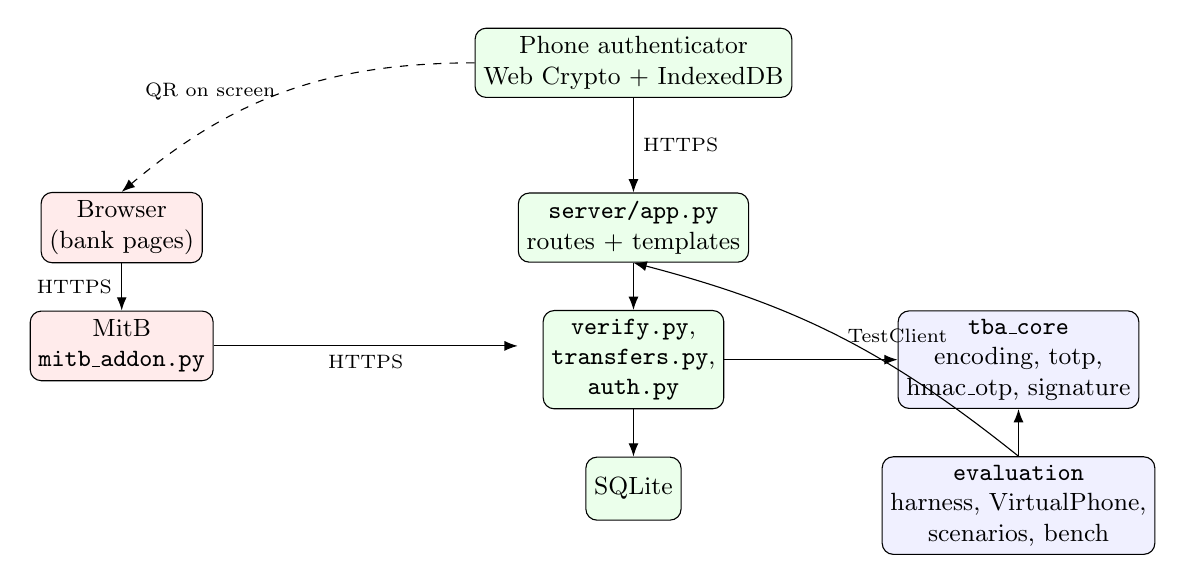
\begin{tikzpicture}[
  font=\small,
  box/.style={draw,rounded corners,align=center,minimum height=8mm,inner sep=3pt},
  trusted/.style={box,fill=green!8},
  untrusted/.style={box,fill=red!8},
  neutral/.style={box,fill=blue!6},
  >=Latex]
  % untrusted PC
  \node[untrusted] (br) {Browser\\(bank pages)};
  \node[untrusted,below=6mm of br] (mitb) {MitB\\\texttt{mitb\_addon.py}};
  % server
  \node[trusted,right=40mm of br] (web) {\texttt{server/app.py}\\routes + templates};
  \node[trusted,below=6mm of web] (ver) {\texttt{verify.py},\\\texttt{transfers.py},\\\texttt{auth.py}};
  \node[trusted,below=6mm of ver] (db) {SQLite};
  % phone
  \node[trusted,above=12mm of web] (app) {Phone authenticator\\Web Crypto + IndexedDB};
  % core / eval
  \node[neutral,right=22mm of ver] (core) {\texttt{tba\_core}\\encoding, totp,\\hmac\_otp, signature};
  \node[neutral,below=6mm of core] (eval) {\texttt{evaluation}\\harness, VirtualPhone,\\scenarios, bench};
  % edges
  \draw[->] (br) -- node[left,font=\scriptsize]{HTTPS} (mitb);
  \draw[->] (mitb.east) -- node[below,font=\scriptsize]{HTTPS} (web.west|-mitb.east);
  \draw[->] (app) -- node[right,font=\scriptsize]{HTTPS} (web);
  \draw[->,dashed] (app.west) to[bend right=20] node[left,font=\scriptsize]{QR on screen} (br.north);
  \draw[->] (web) -- (ver);
  \draw[->] (ver) -- (db);
  \draw[->] (ver) -- (core);
  \draw[->] (eval) -- (core);
  \draw[->] (eval.north) to[bend right=12] node[right,font=\scriptsize]{TestClient} (web.south);
\end{tikzpicture}
\caption{Architecture and trust boundaries (F1). Green: trusted; red: untrusted;
blue: test/verification code. The QR code is the only channel from the
untrusted browser to the trusted phone, and the phone talks to the server on its
own HTTPS channel.}
\label{fig:arch}
\end{figure}

\subsection{Transaction encoding}
A transaction is a fixed JSON object; every field is validated identically in
Python and in JavaScript (\cref{tab:txfields}). The \emph{canonical} form is
\texttt{json.dumps(tx, sort\_keys=True, separators=(",",":"), ensure\_ascii=True)}
encoded as ASCII. Parsing is strict: duplicate keys, floating-point numbers,
\texttt{NaN}/\texttt{Infinity}, non-ASCII bytes, and any string that does not
re-serialise to the identical bytes are rejected. The transaction QR payload is
\texttt{"tba1:"} followed by the base64url of the canonical bytes; the enrolment
QR payload is \texttt{"tbaenroll1:"} followed by a token. The server always
verifies against the canonical transaction stored in \emph{its own} database,
never a transaction sent by the client.

\begin{table}[htbp]
\centering
\caption{Transaction fields and their constraints.}
\label{tab:txfields}
\small
\begin{tabularx}{\linewidth}{@{}lX@{}}
\toprule
Field & Constraint \\
\midrule
\texttt{v}        & integer, equal to 1 \\
\texttt{tx\_id}   & lower-case UUID \texttt{[0-9a-f]\{8\}-...-[0-9a-f]\{12\}} \\
\texttt{from}, \texttt{to} & \texttt{[0-9]\{6,20\}} \\
\texttt{to\_name} & \texttt{[A-Z0-9 ]\{1,64\}} \\
\texttt{amount}   & integer (not bool), $1 \le \texttt{amount} \le 2^{53}-1$ \\
\texttt{currency} & \texttt{[A-Z]\{3\}} \\
\texttt{nonce}    & 16 random bytes, base64url without padding, exactly 22 chars \\
\texttt{exp}      & integer, equal to creation time $+\,120$ seconds \\
\bottomrule
\end{tabularx}
\end{table}

\subsection{The four modes}
\Cref{tab:crypto} gives, for each mode, what the phone computes and what the
server checks. Each device has its own $K_{\text{totp}}$ (20 bytes) and
$K_{\text{hmac}}$ (32 bytes); the ECDSA key pair is generated on the phone. The
domain-separation tags (\texttt{"TBA-HMAC-v1"}, \texttt{"TBA-SIG-v1"}), joined to
the canonical bytes with a \texttt{0x00} byte, stop a code or signature for one
purpose being reused for another.

\begin{table}[htbp]
\centering
\caption{Cryptography of each mode (T4).}
\label{tab:crypto}
\small
\begin{tabularx}{\linewidth}{@{}lXX@{}}
\toprule
Mode & Phone computes & Server checks \\
\midrule
\texttt{baseline} & $\mathrm{HOTP}(K_{\text{totp}},\lfloor t/30\rfloor)$, HMAC-SHA1, 6 digits & window $\pm1$ step; reject step $\le$ last used step \\
\texttt{hmac} & $\mathrm{DT}(\mathrm{HMAC\text{-}SHA256}(K_{\text{hmac}}, \text{tag}\,\|\,\texttt{0x00}\,\|\,\mathrm{canon}(tx)))$, 8 digits & \texttt{hmac.compare\_digest} \\
\texttt{sig} & $\mathrm{ECDSA\text{-}P256\text{-}SHA256}(sk, \text{tag}\,\|\,\texttt{0x00}\,\|\,\mathrm{canon}(tx))$, raw 64 bytes & convert to DER, verify with public key \\
\texttt{sig\_blind} & same as \texttt{sig} & same as \texttt{sig} \\
\bottomrule
\end{tabularx}
\end{table}

\subsection{Device enrolment}
Enrolment (\cref{fig:enroll}) establishes one device per user. Crucially, once a
device exists the server \emph{refuses} to enrol another from a web session
alone: \texttt{GET /enroll} returns 409 and issues no token. Otherwise an
attacker with only a session (A1, or a stolen password) could enrol their own
key and approve every transaction, in every mode. In the demo, re-enrolment
requires wiping the database (\texttt{make reset}); a real system needs an
out-of-band process (\cref{sec:discussion}).

\begin{figure}[htbp]
\centering
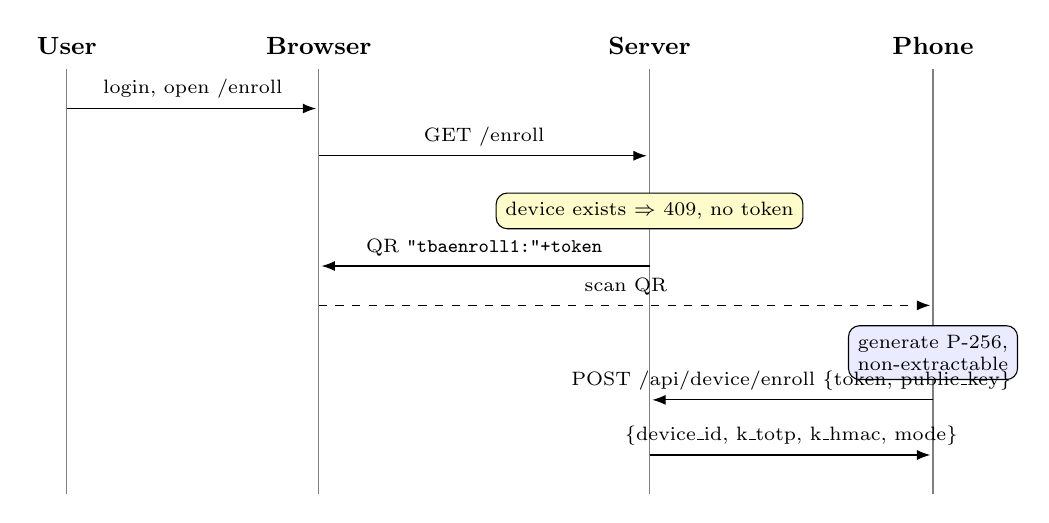
\begin{tikzpicture}[font=\small,>=Latex]
  \def\yl{0}        % top
  \def\yb{-5.4}     % bottom
  \foreach \x/\name in {0/User, 3.2/Browser, 7.4/Server, 11.0/Phone}{
    \node[font=\small\bfseries] at (\x,0.3) {\name};
    \draw[gray] (\x,\yl) -- (\x,\yb);
  }
  \tikzset{msg/.style={->,shorten >=1pt}}
  \draw[msg] (0,-0.5) -- node[above,font=\scriptsize]{login, open /enroll} (3.2,-0.5);
  \draw[msg] (3.2,-1.1) -- node[above,font=\scriptsize]{GET /enroll} (7.4,-1.1);
  \node[align=center,font=\scriptsize,fill=yellow!20,draw,rounded corners] at (7.4,-1.8)
        {device exists $\Rightarrow$ 409, no token};
  \draw[msg] (7.4,-2.5) -- node[above,font=\scriptsize]{QR \texttt{"tbaenroll1:"+token}} (3.2,-2.5);
  \draw[msg,dashed] (3.2,-3.0) -- node[above,font=\scriptsize]{scan QR} (11.0,-3.0);
  \node[align=center,font=\scriptsize,fill=blue!8,draw,rounded corners] at (11.0,-3.6)
        {generate P-256,\\non-extractable};
  \draw[msg] (11.0,-4.2) -- node[above,font=\scriptsize]{POST /api/device/enroll \{token, public\_key\}} (7.4,-4.2);
  \draw[msg] (7.4,-4.9) -- node[above,font=\scriptsize]{\{device\_id, k\_totp, k\_hmac, mode\}} (11.0,-4.9);
\end{tikzpicture}
\caption{Device enrolment (F2). The HMAC keys are sent in the clear over HTTPS
and stored by the phone as non-extractable keys in IndexedDB.}
\label{fig:enroll}
\end{figure}

\subsection{Confirmation under a man-in-the-browser}
\Cref{fig:confirm} shows what happens to a transfer when the browser is
compromised. The MitB rewrites the recipient to the attacker before the request
reaches the server, and masks the returned confirmation page so the browser
still shows the intended recipient. The transaction QR, however, encodes the
transaction the server actually holds, so the phone displays the \emph{true}
recipient. In \texttt{hmac} and \texttt{sig} an attentive user sees the mismatch
and rejects; in \texttt{sig\_blind} the phone shows nothing, so the user cannot
notice. This is the mechanism measured in \cref{sec:eval} and shown in the
screenshots of \cref{fig:mitb}.

\begin{figure}[htbp]
\centering
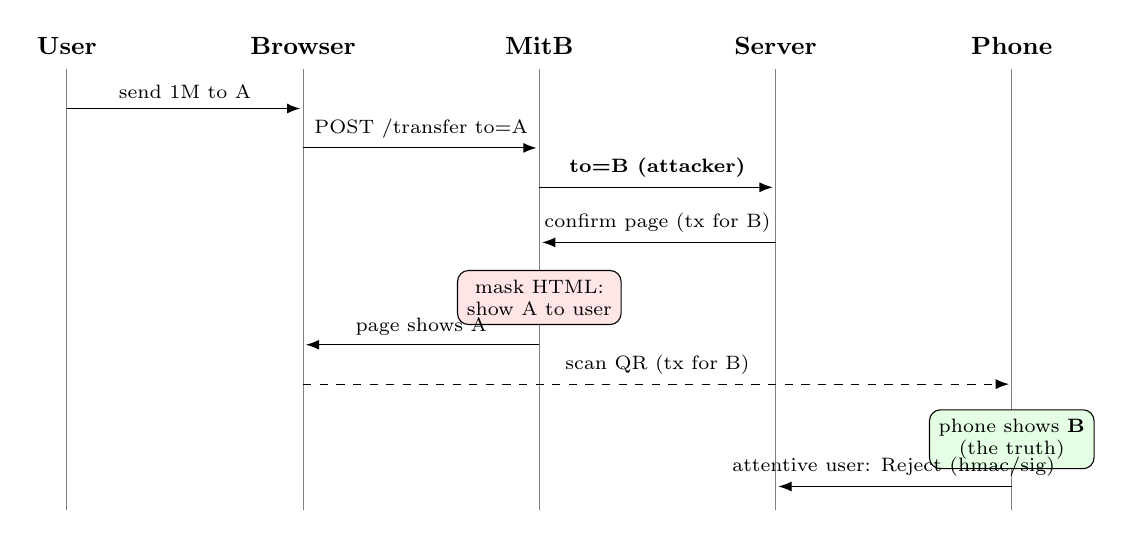
\begin{tikzpicture}[font=\small,>=Latex]
  \foreach \x/\name in {0/User, 3.0/Browser, 6.0/MitB, 9.0/Server, 12.0/Phone}{
    \node[font=\small\bfseries] at (\x,0.3) {\name};
    \draw[gray] (\x,0) -- (\x,-5.6);
  }
  \tikzset{msg/.style={->,shorten >=1pt}}
  \draw[msg] (0,-0.5) -- node[above,font=\scriptsize]{send 1M to A} (3.0,-0.5);
  \draw[msg] (3.0,-1.0) -- node[above,font=\scriptsize]{POST /transfer to=A} (6.0,-1.0);
  \draw[msg] (6.0,-1.5) -- node[above,font=\scriptsize]{\textbf{to=B (attacker)}} (9.0,-1.5);
  \draw[msg] (9.0,-2.2) -- node[above,font=\scriptsize]{confirm page (tx for B)} (6.0,-2.2);
  \node[align=center,font=\scriptsize,fill=red!10,draw,rounded corners] at (6.0,-2.9)
        {mask HTML:\\show A to user};
  \draw[msg] (6.0,-3.5) -- node[above,font=\scriptsize]{page shows A} (3.0,-3.5);
  \draw[msg,dashed] (3.0,-4.0) -- node[above,font=\scriptsize]{scan QR (tx for B)} (12.0,-4.0);
  \node[align=center,font=\scriptsize,fill=green!10,draw,rounded corners] at (12.0,-4.7)
        {phone shows \textbf{B}\\(the truth)};
  \draw[msg] (12.0,-5.3) -- node[above,font=\scriptsize]{attentive user: Reject (hmac/sig)} (9.0,-5.3);
\end{tikzpicture}
\caption{Confirmation under MitB (F3). The browser is deceived, but the phone
reads the transaction the server holds, so \texttt{hmac}/\texttt{sig} expose the
swap. In \texttt{sig\_blind} the phone shows nothing and the user approves.}
\label{fig:confirm}
\end{figure}

\section{Implementation}\label{sec:impl}

The system is a FastAPI server with an SQLite database and Jinja2 templates
(\texttt{server/}), a browser-based phone authenticator built from plain ES
modules (\texttt{authenticator/}), and a shared, I/O-free cryptographic core
(\texttt{tba\_core/}). The server and the phone never share code directly; their
agreement is enforced by a common set of test vectors
(\texttt{shared/vectors.json}) that both a Python test and a Node test check.

\subsection{Canonical encoding}
The security of binding rests on both sides hashing \emph{exactly} the same
bytes. The canonical form fixes key order, removes whitespace, forbids
non-ASCII, and is validated before use:
\begin{lstlisting}[language=Python]
def canonical_bytes(tx: dict) -> bytes:
    validate_tx(tx)
    return json.dumps(tx, sort_keys=True,
                      separators=(",", ":"),
                      ensure_ascii=True).encode("ascii")
\end{lstlisting}
The matching JavaScript produces byte-identical output, which the cross-language
vectors confirm (20 vectors, all passing).

\subsection{Signing on the phone}
The ECDSA key pair is generated in the browser with Web Crypto and is
non-extractable; the signature is taken over the tagged, canonical transaction:
\begin{lstlisting}[language=JavaScript]
export function generateSigningKey() {
  // extractable=false applies to the private key.
  return crypto.subtle.generateKey(
    { name: "ECDSA", namedCurve: "P-256" }, false, ["sign", "verify"]);
}
export async function signTx(privateKey, tx) {
  return new Uint8Array(await crypto.subtle.sign(
    { name: "ECDSA", hash: "SHA-256" },
    privateKey, taggedMessage("TBA-SIG-v1", tx)));
}
\end{lstlisting}
A non-extractable key cannot be exported through the Web Crypto API; this is an
API-level protection, not a hardware one, and it does not prevent the key being
\emph{used} (see the G6 limitation in \cref{sec:threat}).

\subsection{Server-side verification order}
Each confirmation runs inside one \texttt{BEGIN IMMEDIATE} transaction
(\texttt{write\_tx}) so that concurrent submissions of the same code cannot both
succeed (goal~G3). The order is: (1)~the \texttt{tx\_id} exists and belongs to
this user; (2)~its state is \texttt{pending}; (3)~it has not expired, else it
becomes \texttt{expired}; (4)~the transaction is rebuilt from the canonical bytes
in the database; (5)~the OTP or signature is verified --- on failure
\texttt{attempts} is incremented and, at three, the transaction becomes
\texttt{failed}; (6)~on success the balances move, the state becomes
\texttt{executed}, and the OTP or signature is stored as evidence; (7)~an audit
record is written. Evidence of the wrong kind (an OTP in a signature mode, or a
signature in an OTP mode) is rejected before step~1 and does \emph{not} consume
an attempt. The server verifies only the canonical transaction it stored, never
one supplied by the client.

\subsection{The authenticator interface}
\Cref{fig:ui} shows the authenticator's transaction screen. In \texttt{hmac} and
\texttt{sig} it shows the amount, the recipient account and the recipient name
read from the scanned QR; the user compares these with their intent before
approving. (The figure is taken from the man-in-the-browser demo of
\cref{sec:eval}, so the recipient it shows is the attacker's.)

\begin{figure}[htbp]
\centering
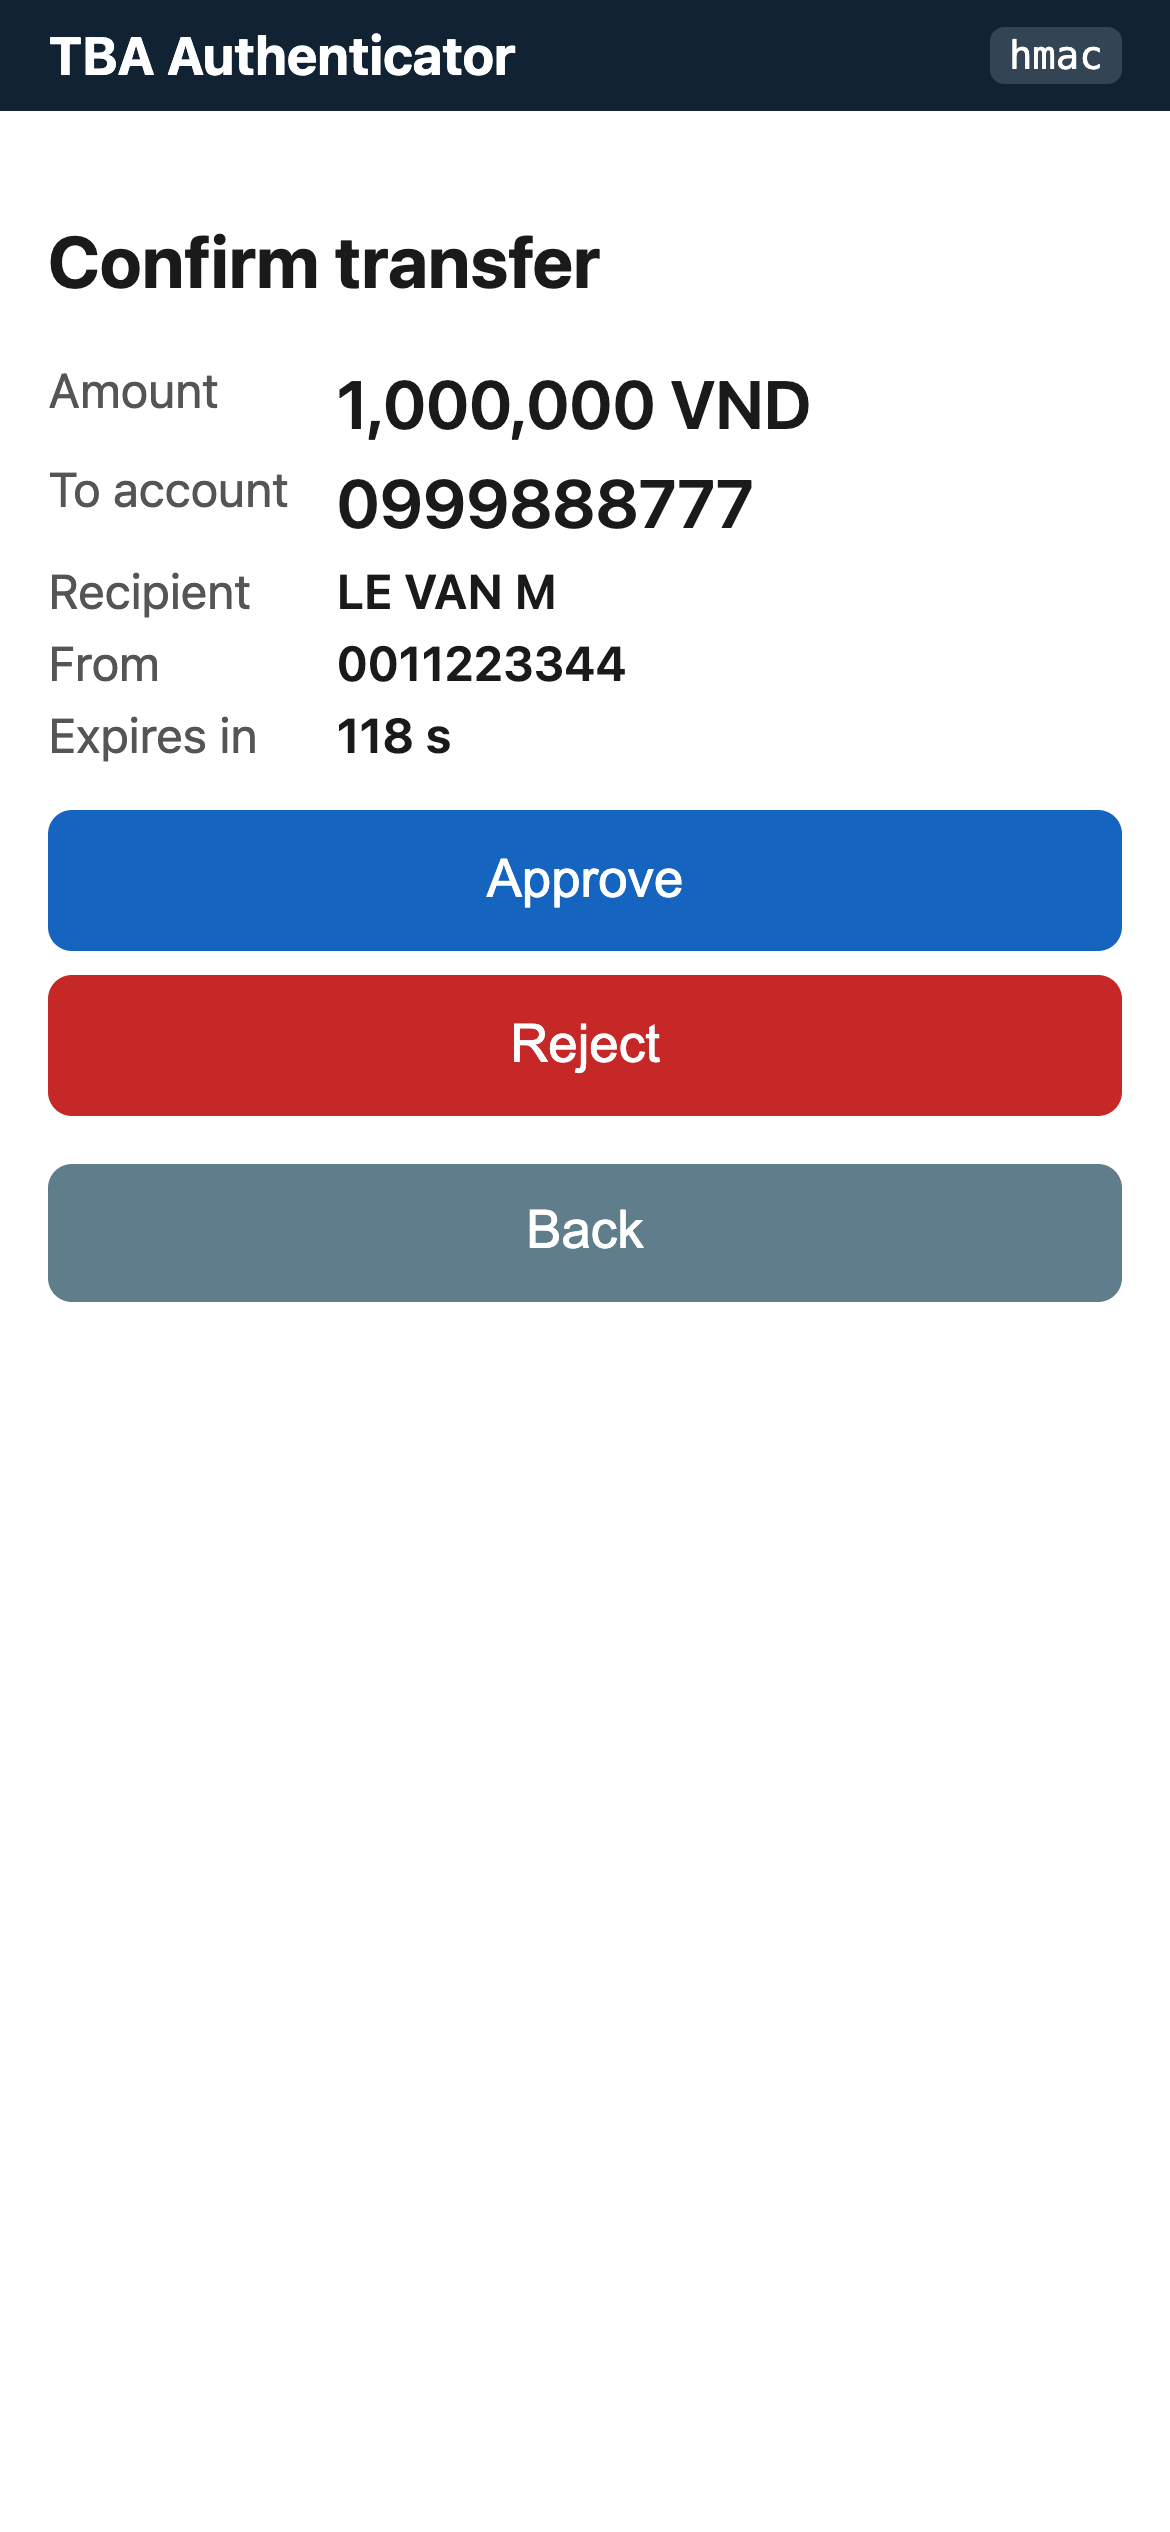
\includegraphics[height=7.5cm]{figures/hmac_phone.png}
\caption{The authenticator's confirmation screen in \texttt{hmac} mode (F7).}
\label{fig:ui}
\end{figure}

\section{Security Evaluation}\label{sec:eval}

\subsection{Methodology}
The evaluation is automated. A \texttt{Lab} builds a fresh in-process server
(with a controllable clock) for each run; a \texttt{VirtualPhone} plays the
authenticator using \texttt{tba\_core}; and a \texttt{Mitb} object rewrites
requests and QR codes exactly as the live \texttt{mitmproxy} addon does. Two user
models bound the human: an \emph{attentive} user approves only when the phone's
display matches their intent (and always approves when the phone shows nothing,
as in blind signing), while a \emph{careless} user always approves. Thirteen
scenarios (S1--S13) are run in all four modes and each outcome is compared with a
pre-declared expected value; \texttt{make scenarios} exits non-zero on any
mismatch. All results below are the committed output of \texttt{make eval} and
live in \texttt{results/}.

\subsection{Case study: man-in-the-browser}
\Cref{fig:mitb} shows the live attack through \texttt{mitmproxy}, for a transfer
the user meant to send to \textbf{TRAN THI B (0123456789)}. The malware rewrites
the recipient to \textbf{LE VAN M (0999888777)}, the attacker's account, and
masks the bank's confirmation page so the laptop still shows TRAN THI B. The
phone, which reads the transaction the server actually holds, tells the truth: in
\texttt{hmac} and \texttt{sig} it shows LE VAN M, so an attentive user rejects; in
\texttt{sig\_blind} it shows no details, so the user approves the theft.

\begin{figure}[htbp]
\centering
\begin{minipage}{0.3\linewidth}\centering
  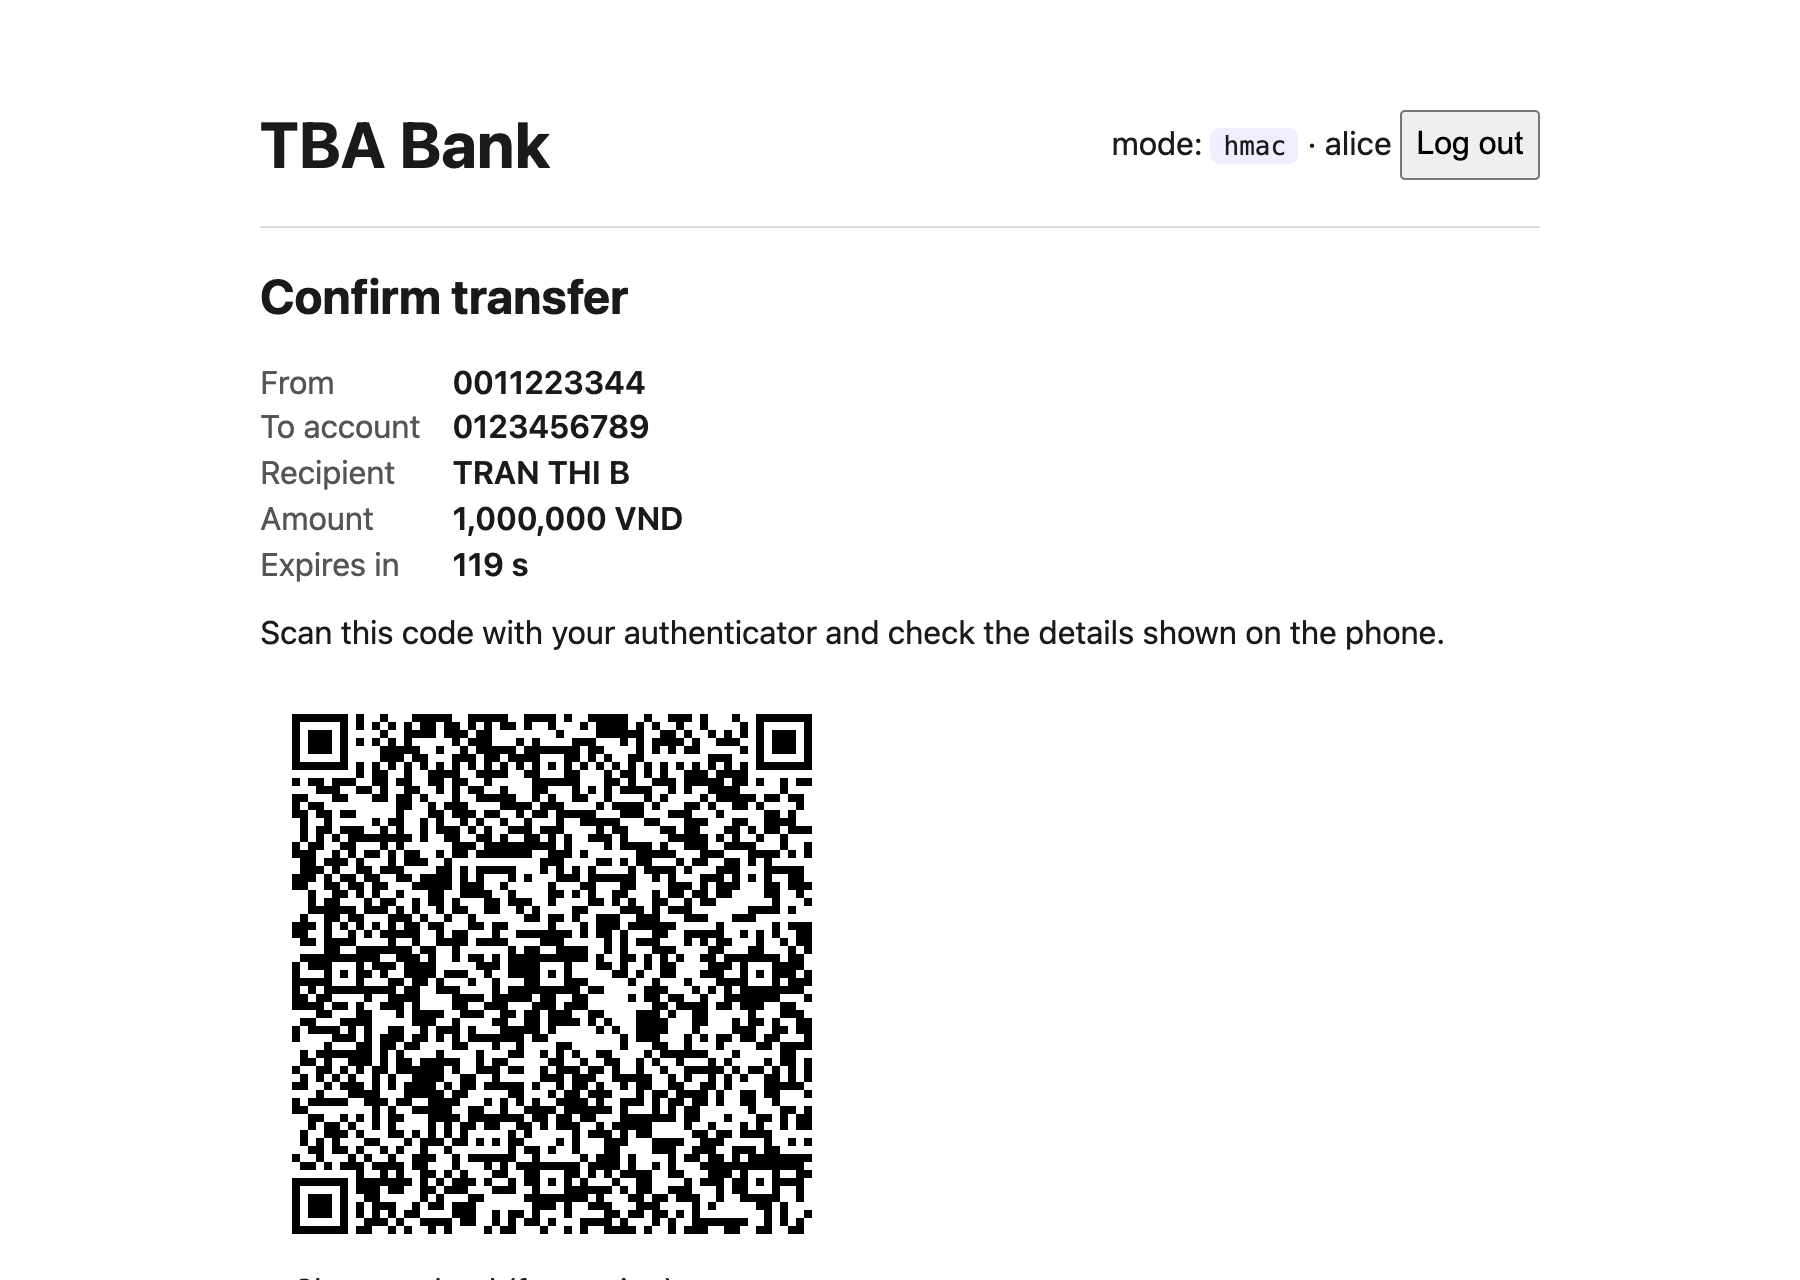
\includegraphics[width=\linewidth]{figures/hmac_laptop.png}\\[1mm]
  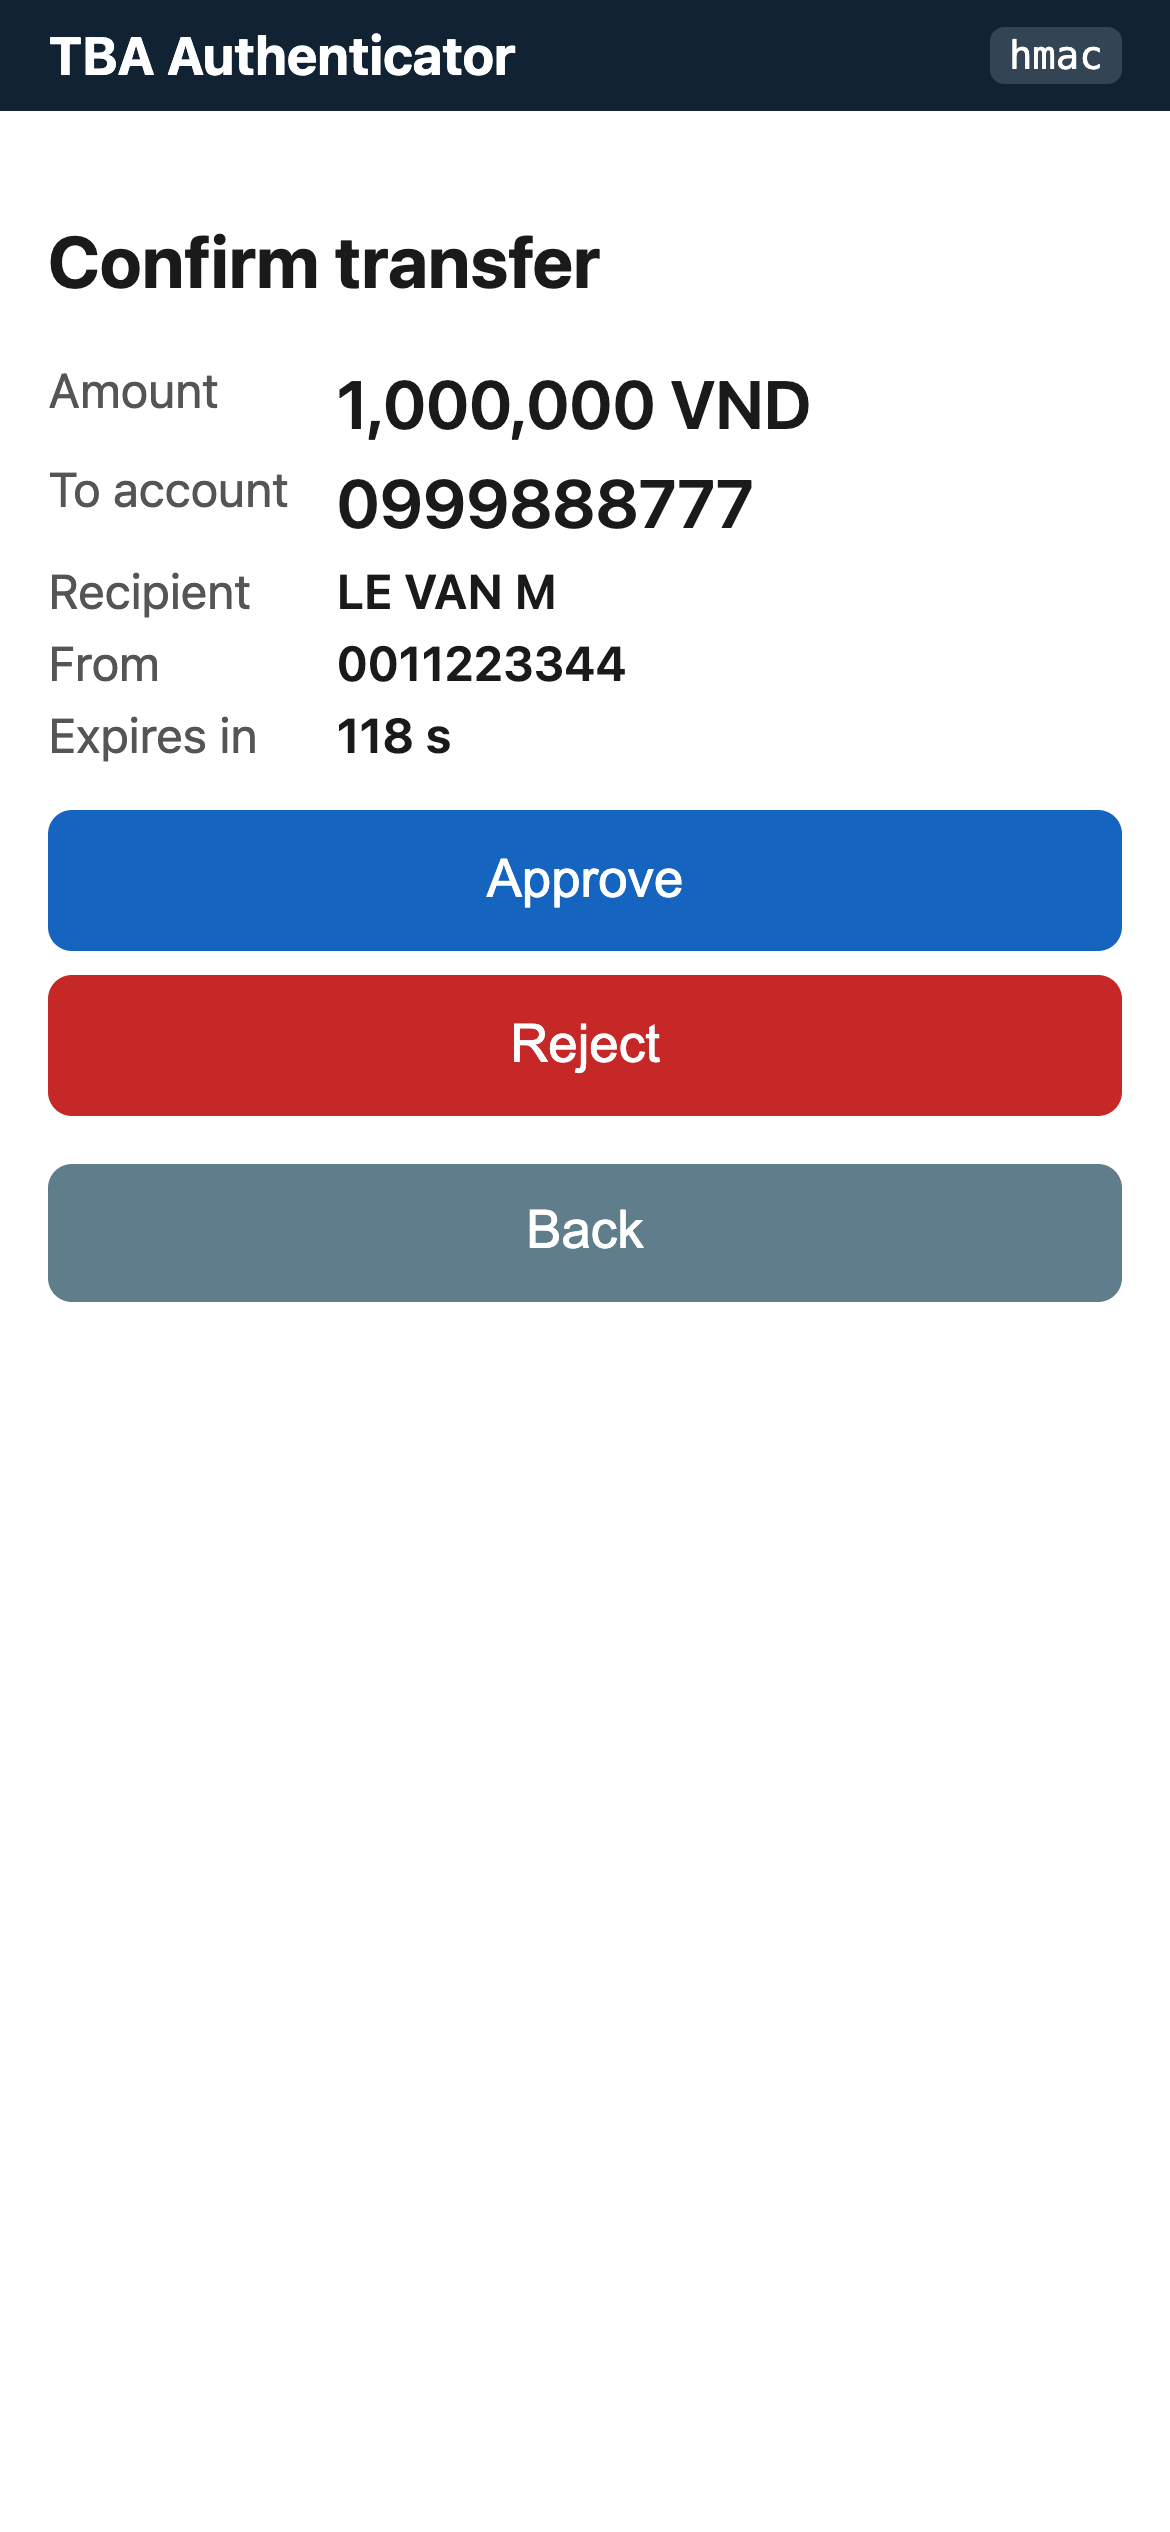
\includegraphics[height=3.4cm]{figures/hmac_phone.png}\\ \footnotesize\texttt{hmac}
\end{minipage}\hfill
\begin{minipage}{0.3\linewidth}\centering
  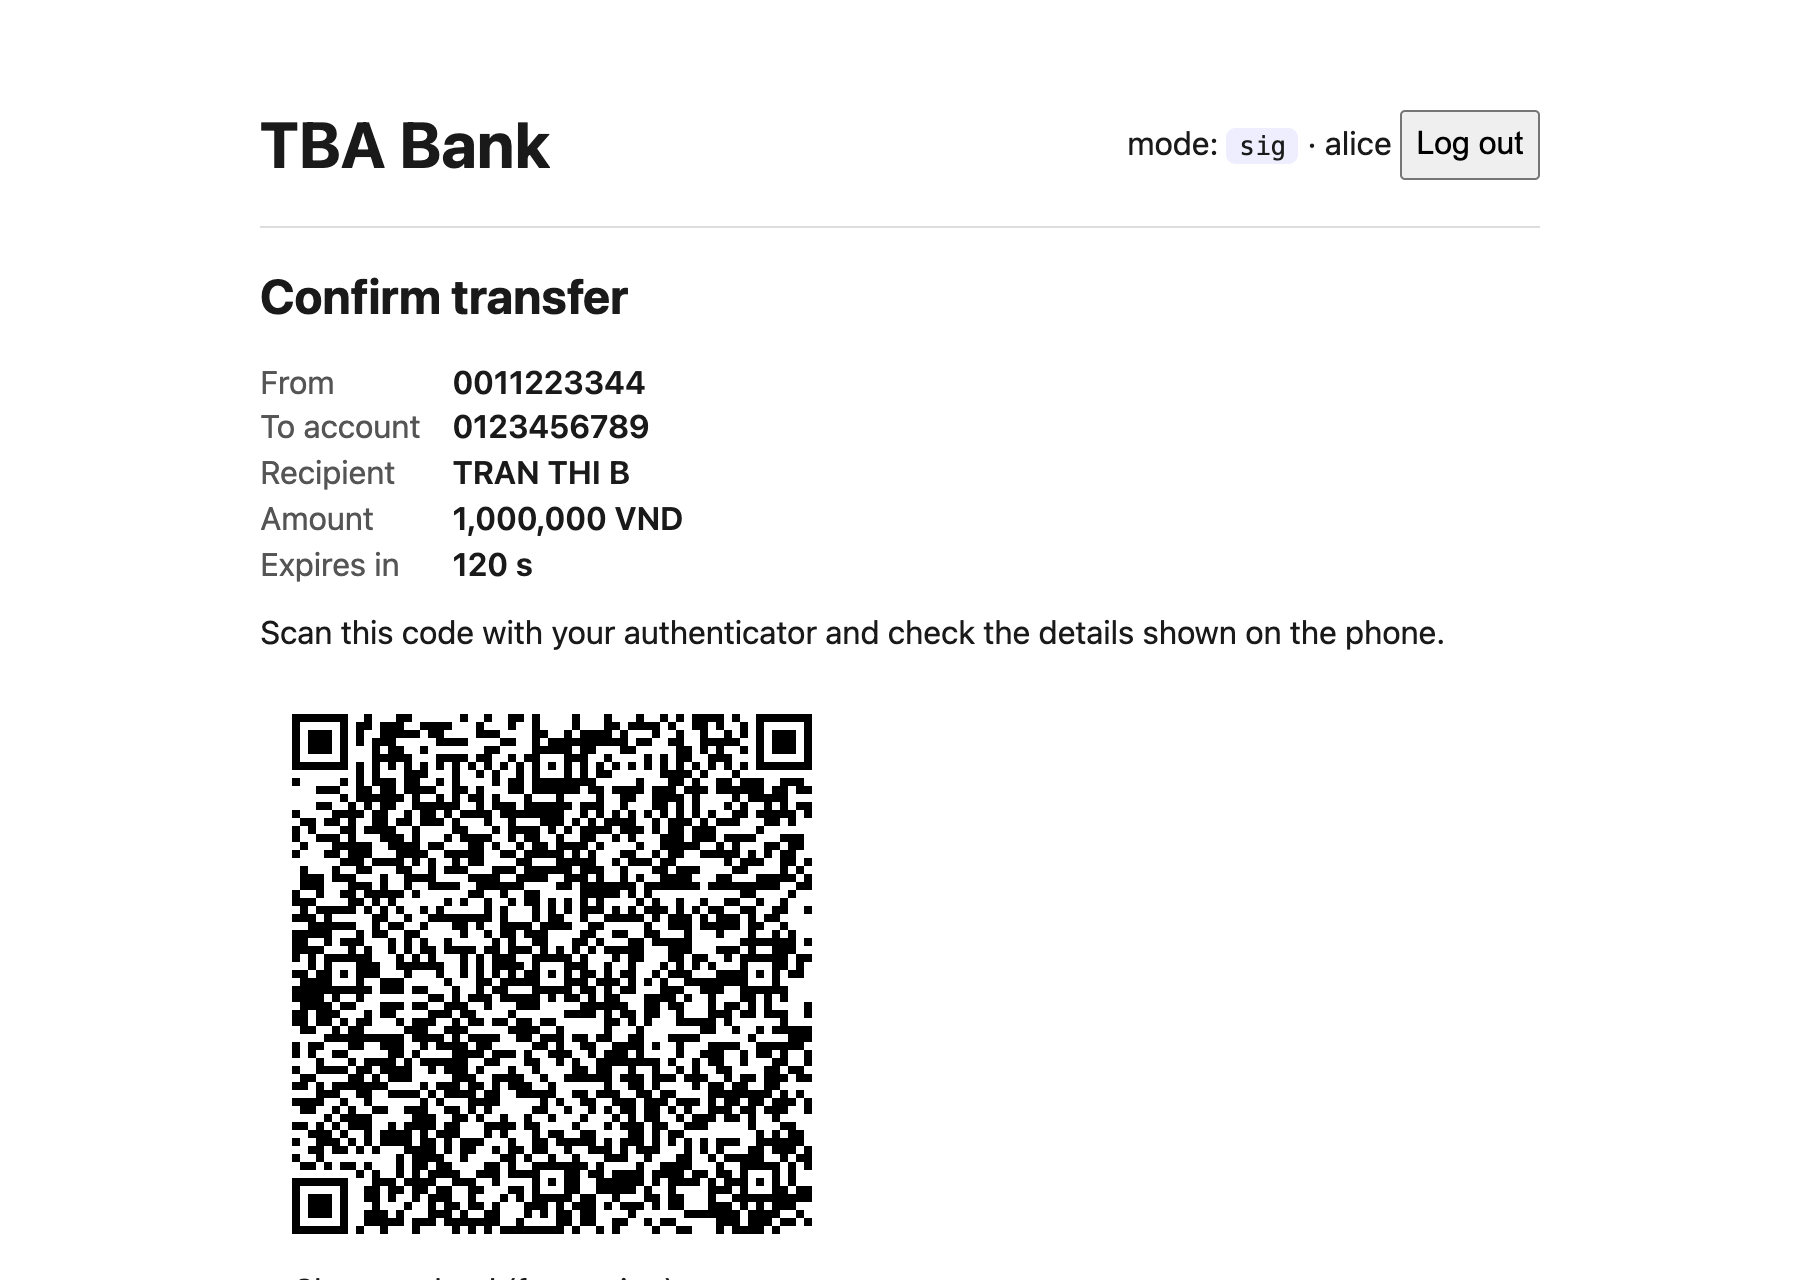
\includegraphics[width=\linewidth]{figures/sig_laptop.png}\\[1mm]
  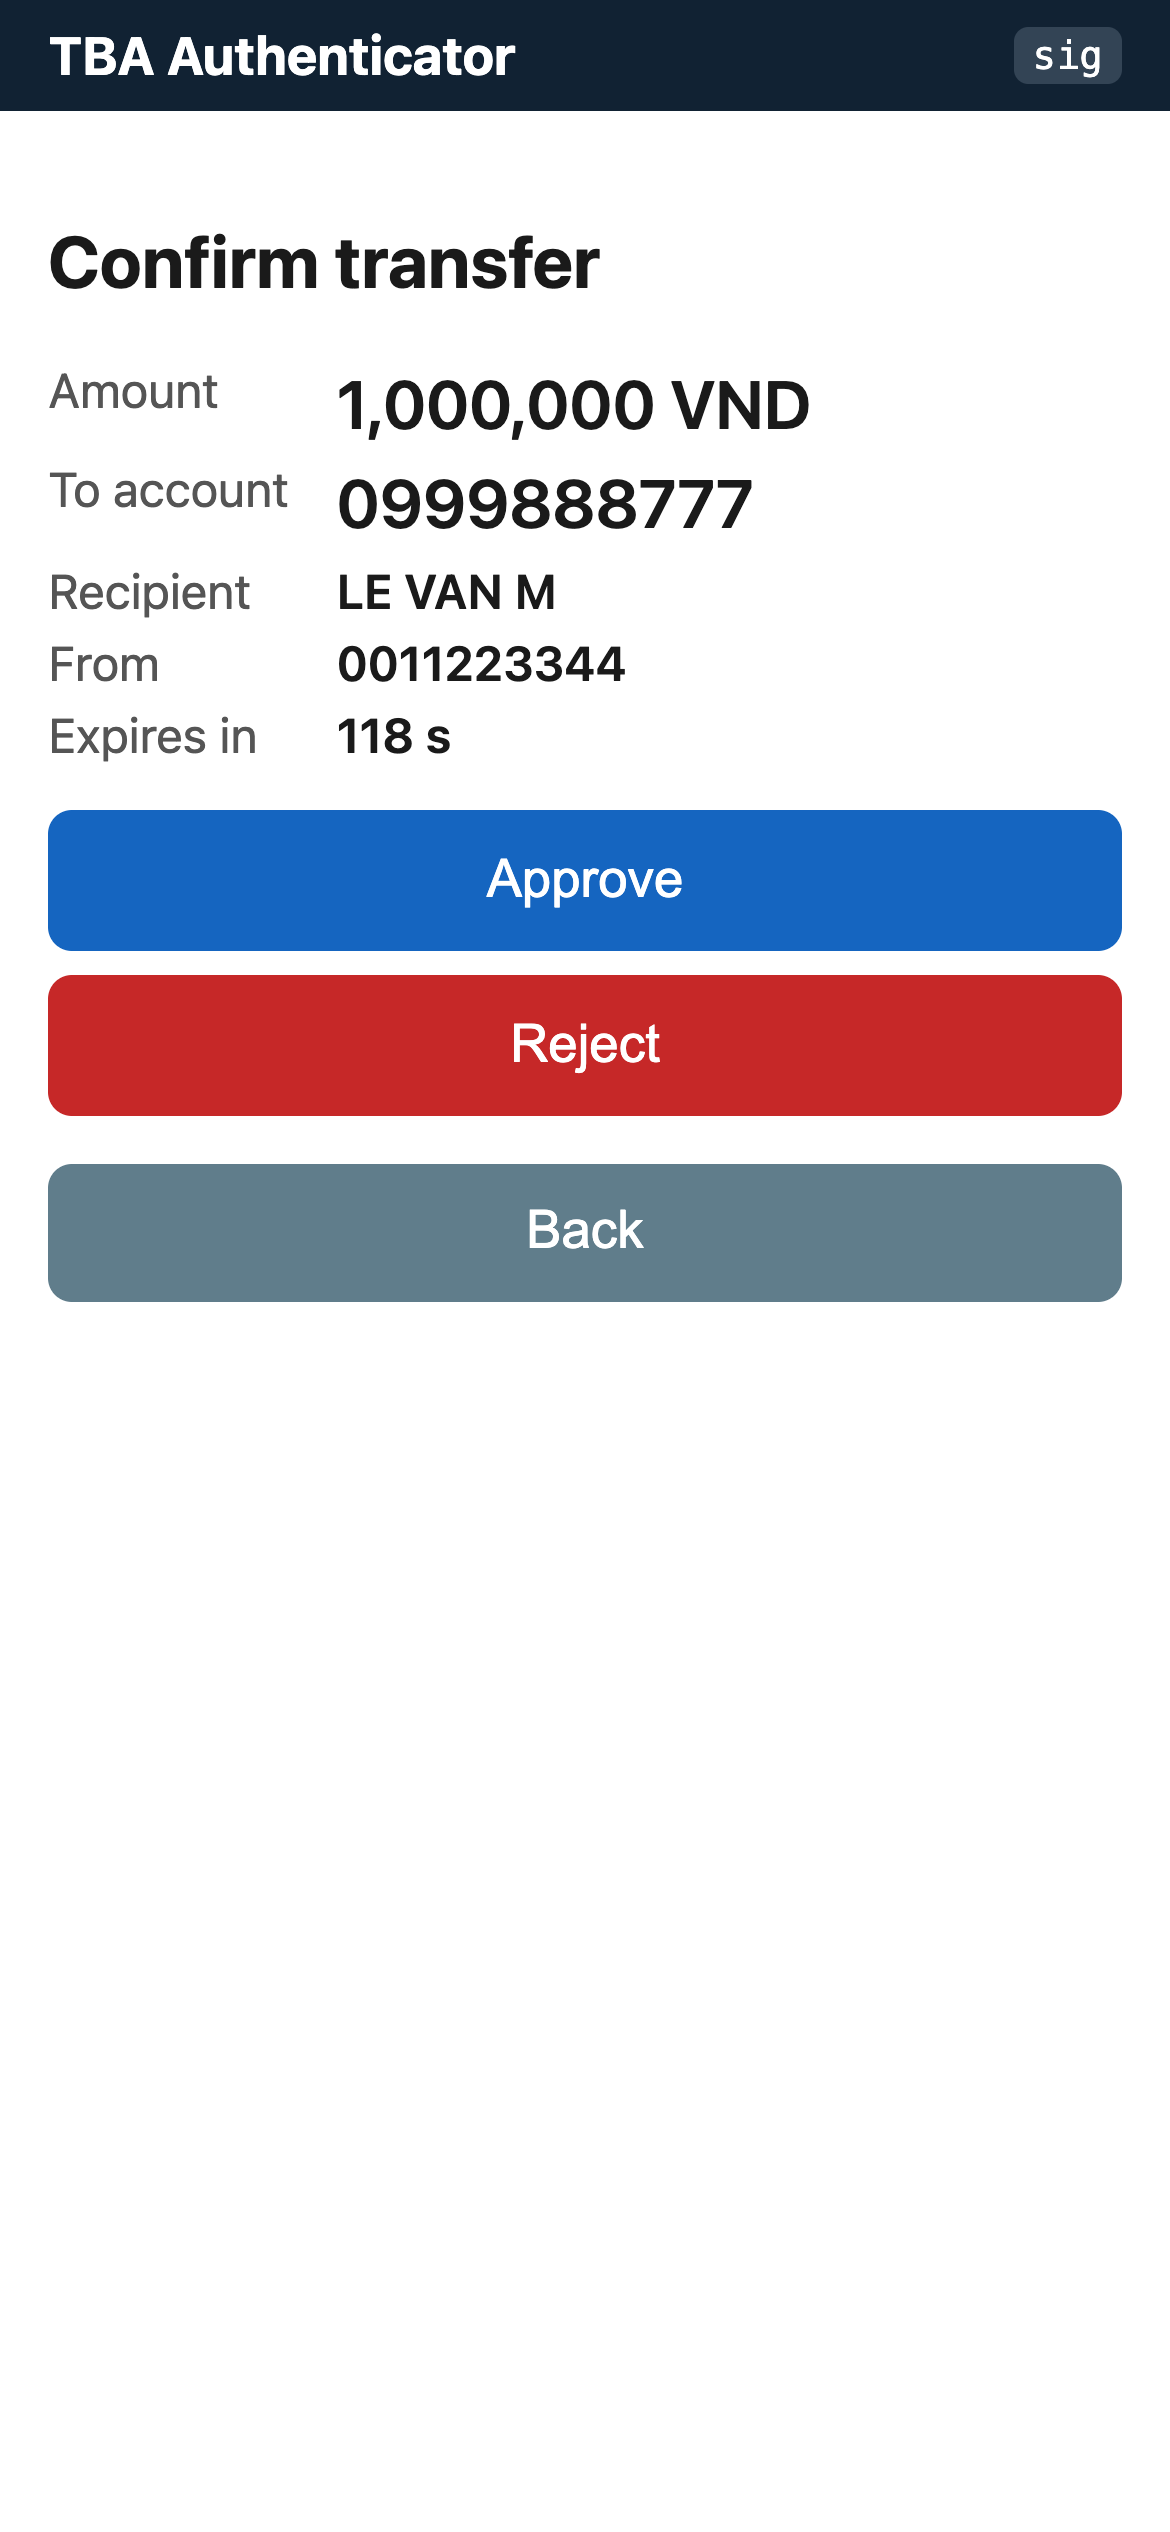
\includegraphics[height=3.4cm]{figures/sig_phone.png}\\ \footnotesize\texttt{sig}
\end{minipage}\hfill
\begin{minipage}{0.3\linewidth}\centering
  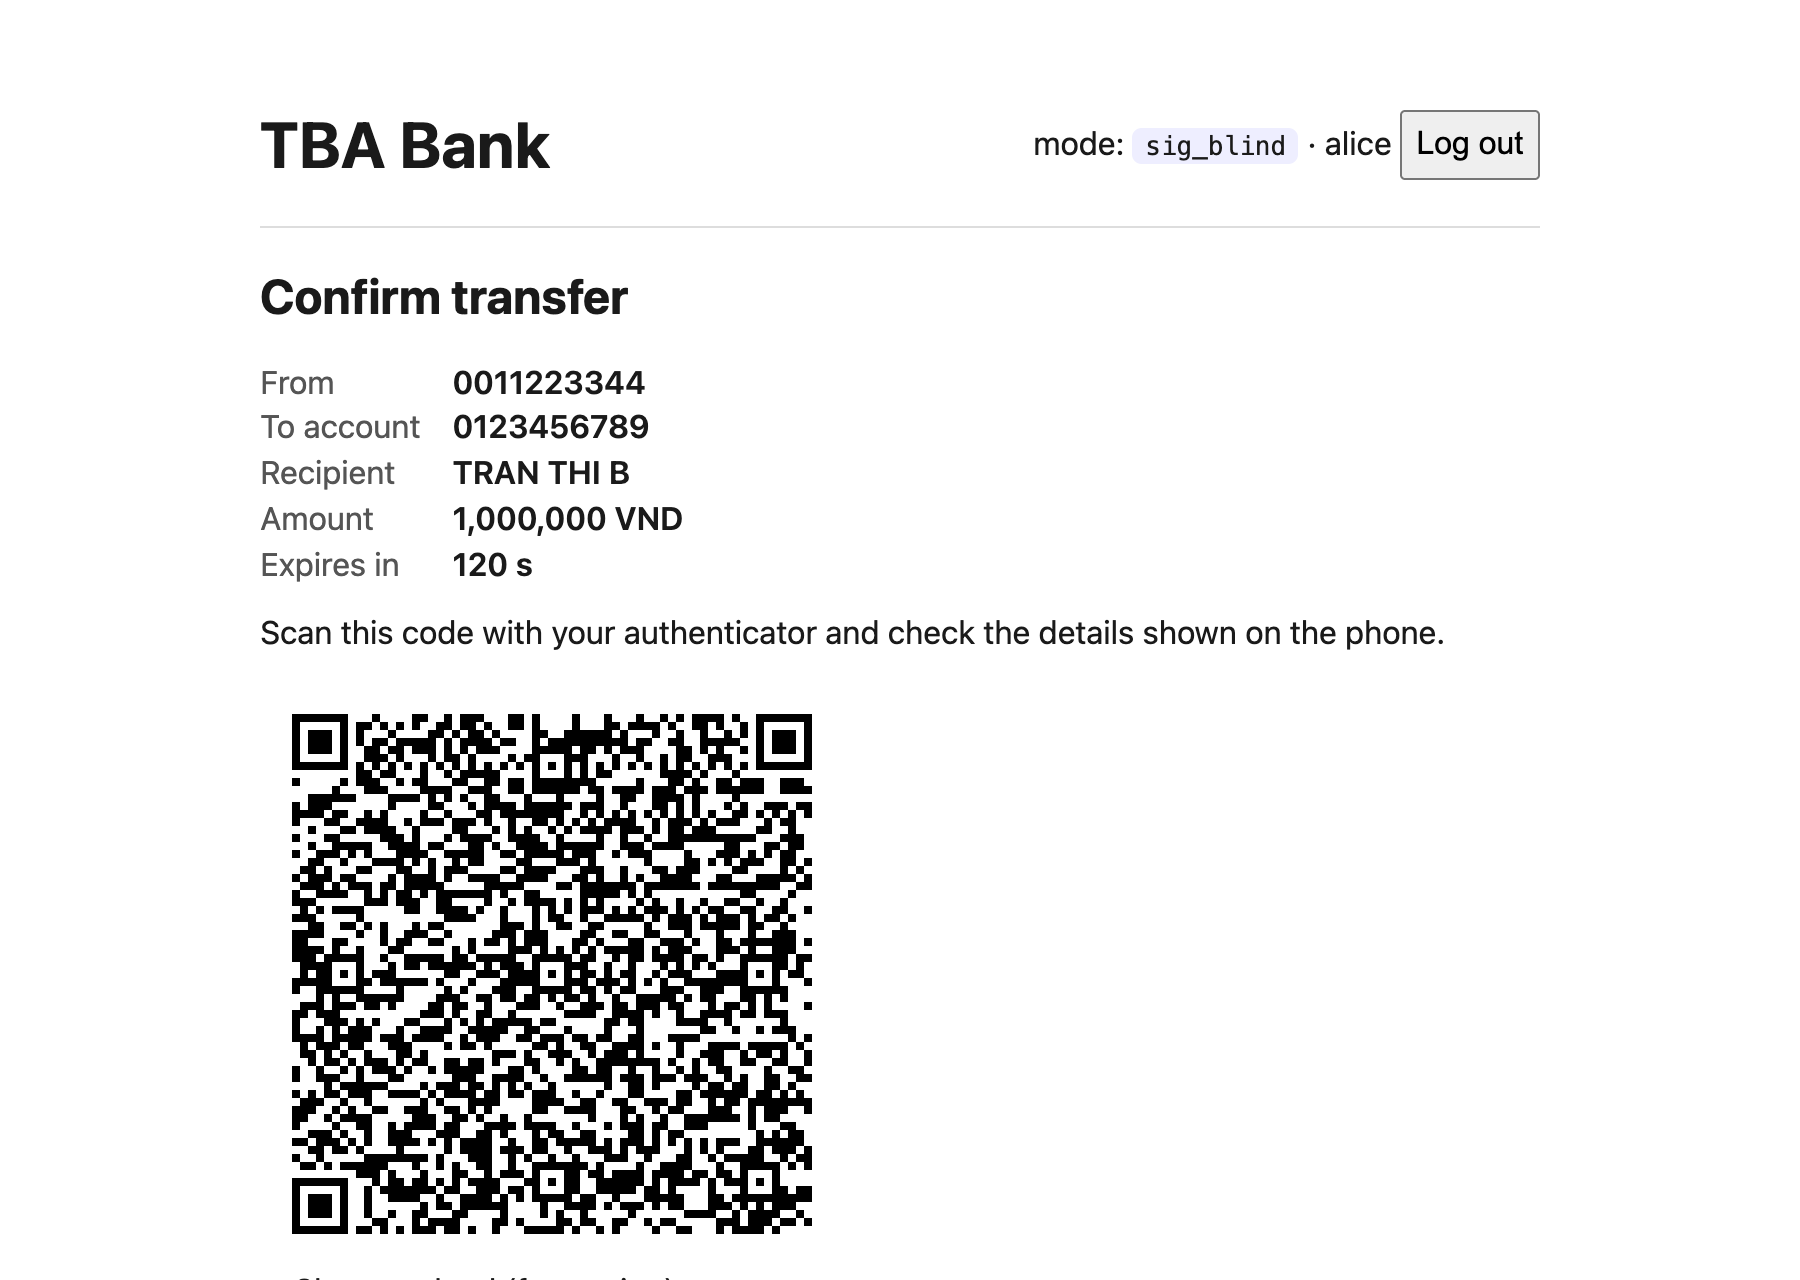
\includegraphics[width=\linewidth]{figures/sig_blind_laptop.png}\\[1mm]
  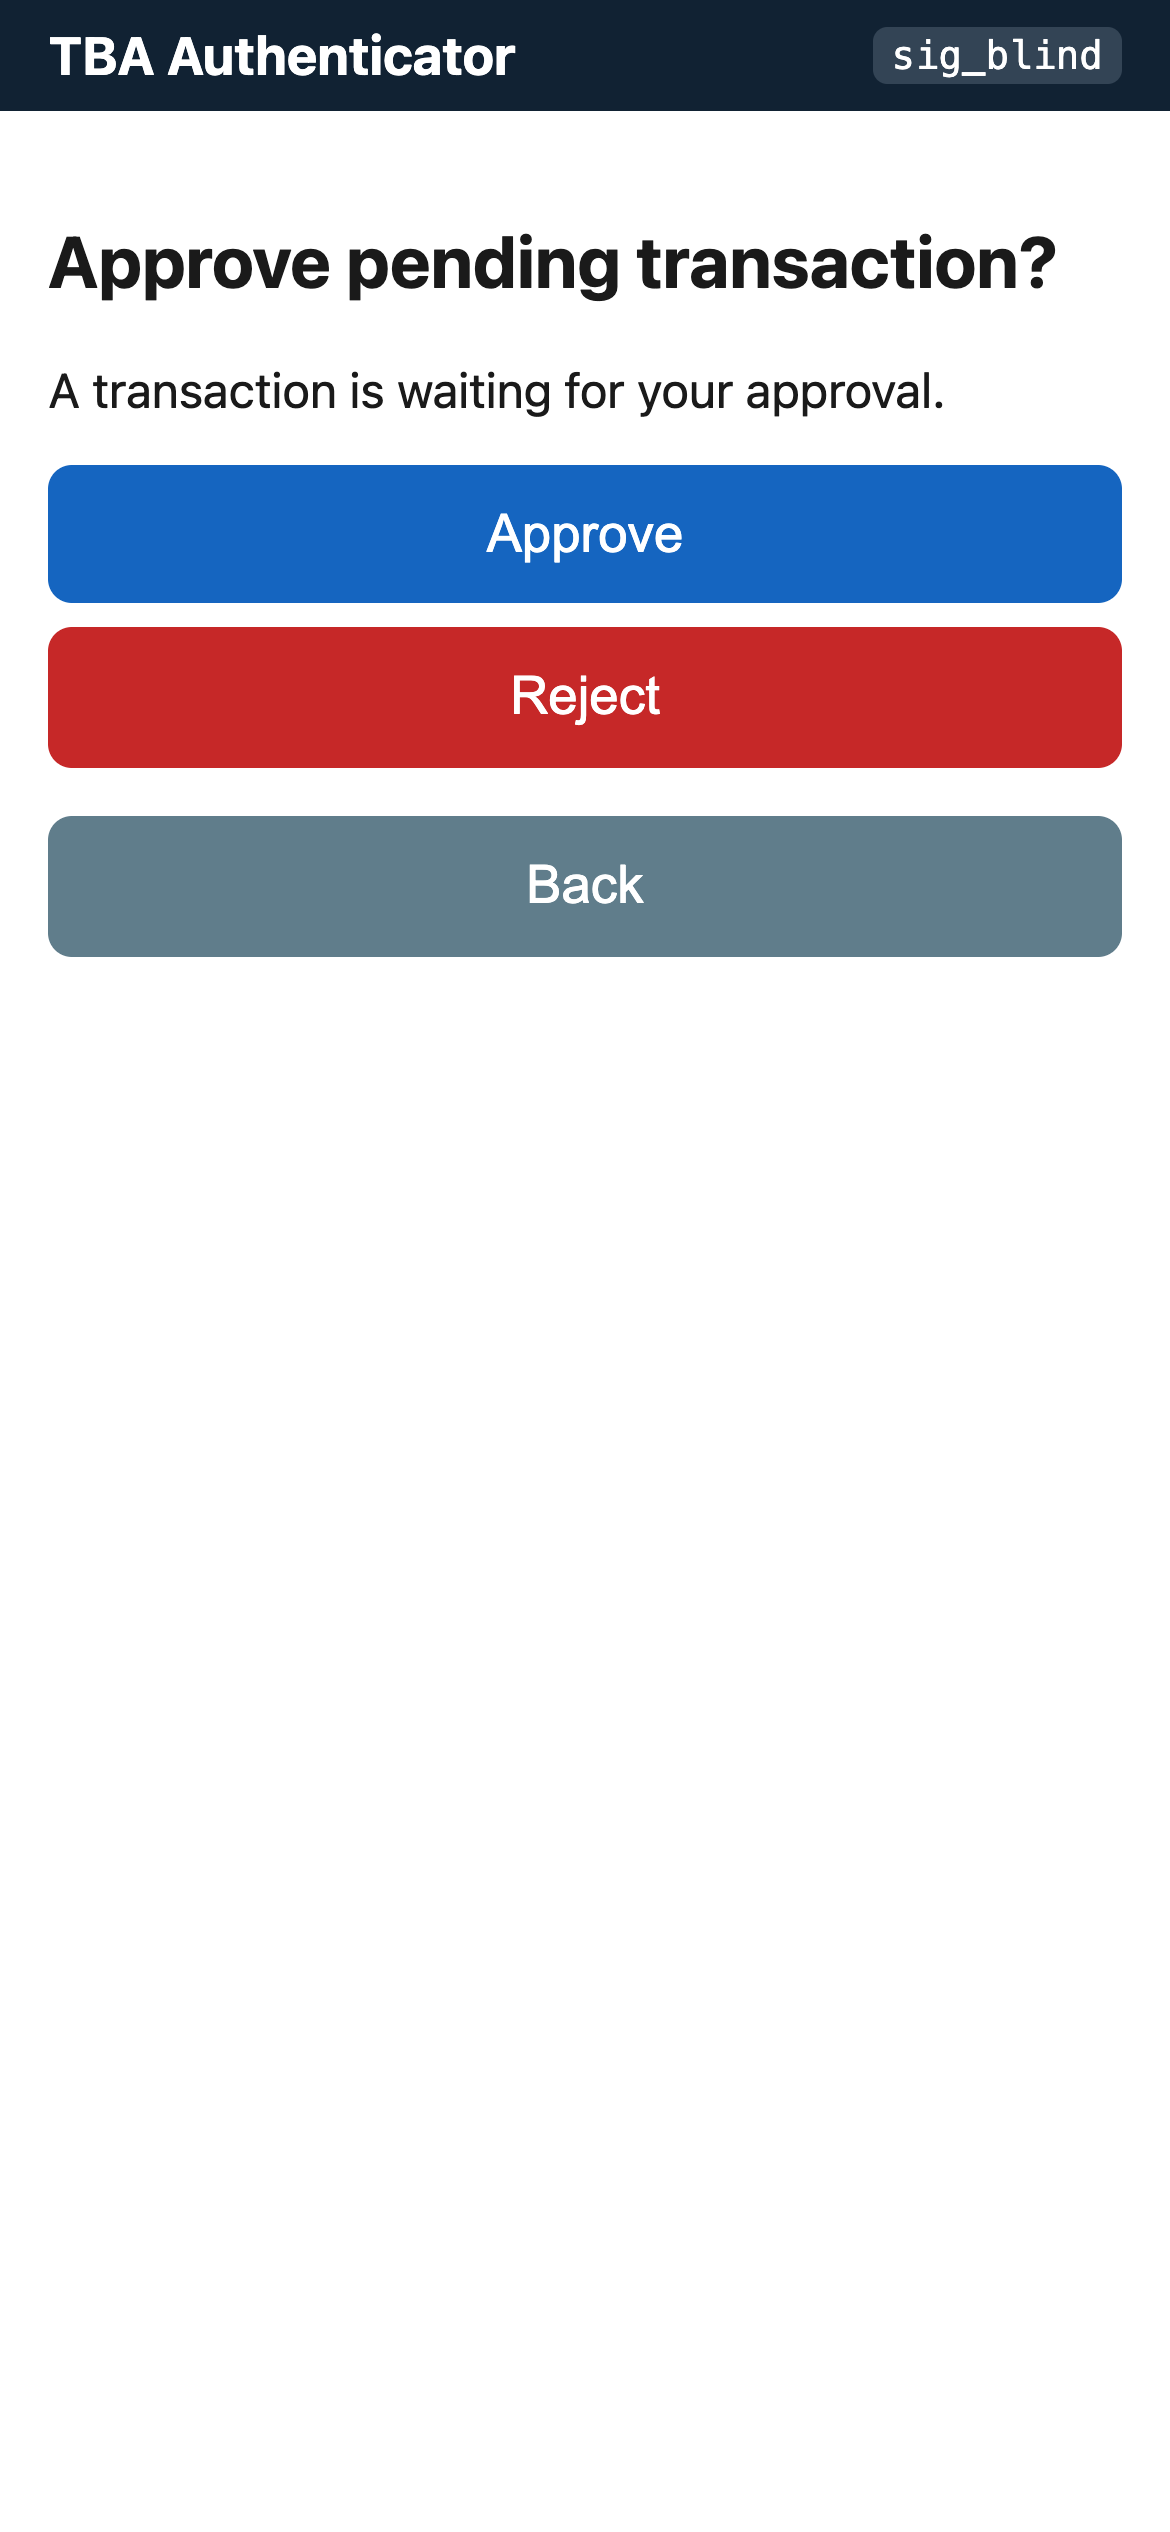
\includegraphics[height=3.4cm]{figures/sig_blind_phone.png}\\ \footnotesize\texttt{sig\_blind}
\end{minipage}
\caption{Live man-in-the-browser (F4). Top row: the laptop confirmation page,
deceived into showing TRAN THI B in every mode. Bottom row: the phone. In
\texttt{hmac}/\texttt{sig} the phone shows the real recipient (0999888777, LE VAN
M); in \texttt{sig\_blind} it shows no details at all.}
\label{fig:mitb}
\end{figure}

\subsection{Scenario results}
\Cref{tab:scenarios} is the full matrix (generated by \texttt{make scenarios};
\cmark{} = secure outcome, \xmark{} = insecure outcome, \texttt{--} = not
applicable). The measured outcomes equal the expected outcomes in all $56$ cells.

\begin{table}[htbp]
\centering
\caption{Scenario outcomes across the four modes (T5). Source:
\texttt{results/scenarios.csv}.}
\label{tab:scenarios}
\small
% --- begin generated content (results/scenarios.tex) ---
\begin{tabularx}{\linewidth}{@{}lXcccc@{}}
\toprule
ID & Scenario & baseline & hmac & sig & sig\_blind \\
\midrule
S1 & Honest transfer & \cmark & \cmark & \cmark & \cmark \\
S2a & MitB swaps recipient, attentive user & \xmark & \cmark & \cmark & \xmark \\
S2b & MitB swaps recipient, careless user & \xmark & \xmark & \xmark & \xmark \\
S3 & MitB changes amount & \xmark & \cmark & \cmark & \xmark \\
S4 & MitB forges QR with intended details & \xmark & \cmark & \cmark & \cmark \\
S5 & Tamper each field after code issued & \xmark & \cmark & \cmark & \cmark \\
S6 & Replay code on old and new transaction & \cmark & \cmark & \cmark & \cmark \\
S7 & Confirm after expiry & \cmark & \cmark & \cmark & \cmark \\
S8 & 50 concurrent submissions of one code & \cmark & \cmark & \cmark & \cmark \\
S9 & 3 wrong guesses, then correct code & \cmark & \cmark & \cmark & \cmark \\
S10 & Server DB leak, forge transfer & \xmark & \xmark & \cmark & \cmark \\
S11 & Third party can verify evidence & \xmark & \xmark & \cmark & \cmark$^{*}$ \\
S12 & Non-canonical QR payloads & -- & \cmark & \cmark & \cmark \\
S13 & Malformed signatures & -- & -- & \cmark & \cmark \\
\bottomrule
\end{tabularx}
\par\smallskip{\footnotesize $^{*}$ In \texttt{sig\_blind} the signature only proves that the device signed, not that the user saw the transaction.\par}
% --- end generated content ---
\end{table}

The matrix answers the research questions directly. Binding the code to the
transaction (\texttt{hmac}, \texttt{sig}) blocks the recipient and amount swaps
(S2a, S3) that \texttt{baseline} lets through, and both block tampering with any
field after the code is issued (S4, S5) --- this is RQ1. The difference between
\texttt{hmac} and \texttt{sig} appears in S10 and S11 (RQ2, \cref{sec:eval-dbleak}).
The difference between \texttt{sig} and \texttt{sig\_blind} appears in S2a and S3
(RQ3): identical cryptography, but without the trusted display the attentive
user has nothing to check, so the swaps succeed. S2b (the careless user) is
\xmark{} everywhere: no cryptography saves a user who approves blindly.

\paragraph{Reading S2a, S3 and G7 (upper bound).}
The \cmark{} cells of S2a and S3, and the \cmark{} for G7, assume the
\emph{attentive} user: they say the mechanism \emph{lets} the user detect the
swap, not that a real user \emph{will}. Real users lie between the attentive and
careless models (\cref{sec:background}); S2b is the lower bound. We do not infer
a detection rate from our own tests.

\subsection{Online guessing}
Scenario S9 confirms that three wrong guesses lock a transaction. To quantify the
residual chance, \texttt{evaluation/bruteforce.py} simulates 100{,}000
transactions with three guesses each, for 3- and 4-digit codes, and compares the
empirical per-transaction success probability with theory
($3/10^d$ for \texttt{hmac}; $1-\binom{10^d-3}{3}/\binom{10^d}{3}$ for
\texttt{baseline}'s three-code window), then extrapolates to 6 and 8 digits
(\cref{tab:bruteforce}, \cref{fig:bruteforce}). Every 95\% confidence interval
contains the theoretical value.

\begin{table}[htbp]
\centering
\caption{Per-transaction guessing probability (T, from
\texttt{results/bruteforce.csv}). 6- and 8-digit rows are theoretical.}
\label{tab:bruteforce}
\small
\begin{tabular}{@{}llrll@{}}
\toprule
Scheme & Digits & Trials & Empirical [95\% CI] & Theory \\
\midrule
\texttt{hmac}     & 3 & 100{,}000 & $0.00279$ $[0.00248, 0.00314]$ & $3.0\times10^{-3}$ \\
\texttt{hmac}     & 4 & 100{,}000 & $0.00030$ $[0.00021, 0.00043]$ & $3.0\times10^{-4}$ \\
\texttt{hmac}     & 6 & --        & --                              & $3.0\times10^{-6}$ \\
\texttt{hmac}     & 8 & --        & --                              & $3.0\times10^{-8}$ \\
\texttt{baseline} & 3 & 100{,}000 & $0.00886$ $[0.00830, 0.00946]$ & $9.0\times10^{-3}$ \\
\texttt{baseline} & 4 & 100{,}000 & $0.00085$ $[0.00069, 0.00105]$ & $9.0\times10^{-4}$ \\
\texttt{baseline} & 6 & --        & --                              & $9.0\times10^{-6}$ \\
\texttt{baseline} & 8 & --        & --                              & $9.0\times10^{-8}$ \\
\bottomrule
\end{tabular}
\end{table}

\begin{figure}[htbp]
\centering
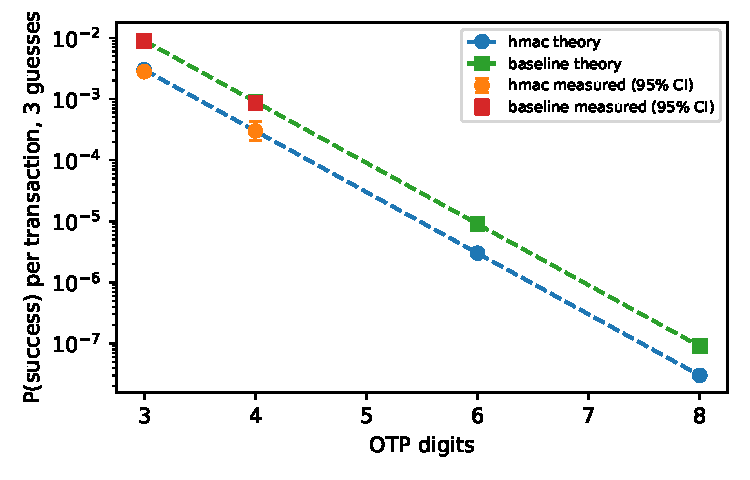
\includegraphics[width=0.75\linewidth]{figures/bruteforce.pdf}
\caption{Empirical vs theoretical guessing probability (F5).}
\label{fig:bruteforce}
\end{figure}

\paragraph{Limitation of G4 (per-transaction only).}
The three-attempt limit is per transaction; there is no per-user counter and
transaction creation is not rate-limited (\cref{sec:threat}). An attacker with
the password but no phone can create $k$ transactions and guess three times each,
so the cumulative success probability is about $k\cdot p$. At the deployed digit
counts this means roughly $7.7\times10^{4}$ transactions for a 50\% chance
against \texttt{baseline} (6 digits, $p\approx9.0\times10^{-6}$) and about
$2.3\times10^{7}$ against \texttt{hmac} (8 digits, $p=3.0\times10^{-8}$);
\texttt{sig}/\texttt{sig\_blind} cannot be guessed at all, as the attacker would
have to forge an ECDSA signature. The \cmark{} for G4 therefore means only that
the per-transaction lockout works. A per-user or per-device failure counter and a
rate limit on transaction creation would close the gap, at the cost of letting an
attacker who knows the password lock the victim out on purpose (a denial of
service).

\subsection{Server compromise and verifiable evidence}
\label{sec:eval-dbleak}
Scenarios S10 and S11 separate \texttt{hmac} from \texttt{sig}. In S10 the
attacker holds a copy of the database and tries to forge a transfer. Because the
server stores $K_{\text{totp}}$ and $K_{\text{hmac}}$ in the clear (deliberately,
to make this scenario real), an attacker with the database can compute valid
\texttt{baseline} and \texttt{hmac} codes --- so both are \xmark{}. The signing
key, by contrast, never leaves the phone, so the leaked database contains only
public keys and \texttt{sig}/\texttt{sig\_blind} remain \cmark{}. A real system
would protect the symmetric keys in an HSM; we did not, in order to demonstrate
exactly this difference.

S11 asks whether a third party can verify the stored evidence. For
\texttt{baseline} and \texttt{hmac} the evidence is a symmetric OTP, checkable
only by whoever holds the key, so the answer is \emph{no}. For \texttt{sig} the
evidence is a signature any party can verify with the public key, so the answer
is \emph{yes}. For \texttt{sig\_blind} the answer is \emph{yes} with the
asterisk: the signature proves the device signed, not that the user saw the
transaction. As set out in \cref{sec:threat}, this is \emph{verifiable evidence},
not non-repudiation: the authenticator is served by the bank, and the public key
is attested by no independent party.

\subsection{Summary against security goals}
\Cref{tab:goalsummary} collapses the scenario matrix onto the seven goals
(generated by \texttt{make scenarios}).

\begin{table}[htbp]
\centering
\caption{Security goals met by each mode (T6). Source: derived from
\texttt{results/scenarios.csv}.}
\label{tab:goalsummary}
\small
% --- begin generated content (results/goals.tex) ---
\begin{tabularx}{\linewidth}{@{}lXcccc@{}}
\toprule
Goal & Description & baseline & hmac & sig & sig\_blind \\
\midrule
G1 & Authorization integrity (code bound to the exact transaction) & \xmark & \cmark & \cmark & \cmark \\
G2 & Freshness (no replay, no late use) & \cmark & \cmark & \cmark & \cmark \\
G3 & Single use under concurrency & \cmark & \cmark & \cmark & \cmark \\
G4 & Guessing limit per transaction & \cmark & \cmark & \cmark & \cmark \\
G5 & Resilience to server database leak & \xmark & \xmark & \cmark & \cmark \\
G6 & Verifiable evidence (third party can check) & \xmark & \xmark & \cmark & \cmark$^{*}$ \\
G7 & What you see is what you sign (attentive user) & \xmark & \cmark & \cmark & \xmark \\
\bottomrule
\end{tabularx}
\par\smallskip{\footnotesize $^{*}$ In \texttt{sig\_blind} the signature only proves that the device signed, not that the user saw the transaction.\par}
% --- end generated content ---
\end{table}

\section{Performance}\label{sec:perf}

All micro-benchmarks were produced by \texttt{make bench} and \texttt{make
sizes} on the machine recorded in \texttt{results/bench\_env.json}: an
\texttt{arm64} macOS host, Python~3.15.2, \texttt{cryptography}~50.0.2 over
OpenSSL~4.0.3.

\subsection{P1: operation latency on the host}
\Cref{tab:bench} gives the median and 95th-percentile time of each operation over
10{,}000 runs (\texttt{results/bench.csv}). Every operation is cheap. ECDSA~P-256
signing is about $19\,\mu s$ and verification about $49\,\mu s$; the HMAC code is
about $5\,\mu s$. Ed25519 is shown for comparison only (it is not used by any
mode): it signs more slowly but with similarly small cost.

\begin{table}[htbp]
\centering
\caption{Operation latency on the host (P1, T7). Source:
\texttt{results/bench.csv}.}
\label{tab:bench}
\small
\begin{tabular}{@{}lrr@{}}
\toprule
Operation & Median ($\mu s$) & p95 ($\mu s$) \\
\midrule
\texttt{canonical\_encode}   & 3.50  & 3.71 \\
\texttt{totp}                & 1.62  & 1.75 \\
\texttt{hmac\_otp}           & 5.25  & 5.42 \\
\texttt{hmac\_otp\_verify}   & 5.42  & 5.58 \\
\texttt{ecdsa\_p256\_sign}   & 19.17 & 19.96 \\
\texttt{ecdsa\_p256\_verify} & 48.50 & 51.04 \\
\texttt{ed25519\_sign}       & 26.67 & 27.79 \\
\texttt{ed25519\_verify}     & 67.96 & 76.29 \\
\bottomrule
\end{tabular}
\end{table}

\begin{figure}[htbp]
\centering
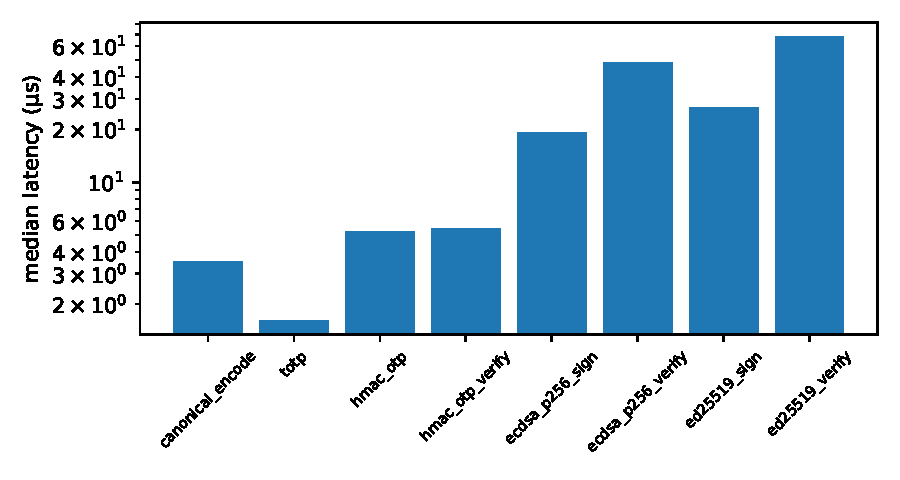
\includegraphics[width=0.75\linewidth]{figures/bench.pdf}
\caption{Operation latency on the host (F6).}
\label{fig:bench}
\end{figure}

\subsection{P2: signing on a real phone}
\Cref{tab:phone} reports the signing time measured in the authenticator itself on
two phones (200 signatures each, \texttt{results/phone\_bench.csv}). Safari on
iOS coarsens \texttt{performance.now()} to 1\,ms, so the per-sample median and
p95 read as 0 and 1\,ms and are not meaningful; the reliable figure is the mean
over the whole run, which is well under a millisecond on both devices. Signing
cost is therefore negligible next to the time the user spends scanning the QR and
reading the screen.

\begin{table}[htbp]
\centering
\caption{ECDSA P-256 signing on real phones (P2, T8). Source:
\texttt{results/phone\_bench.csv}. Median/p95 are limited by Safari's 1\,ms clock.}
\label{tab:phone}
\small
\begin{tabular}{@{}llrrrr@{}}
\toprule
Device & Browser & $n$ & Mean (ms) & Median (ms) & p95 (ms) \\
\midrule
iPhone Air & Safari 26.5 & 200 & 0.290 & 0.00 & 1.00 \\
iPhone 13  & Safari 26.4 & 200 & 0.415 & 0.00 & 1.00 \\
\bottomrule
\end{tabular}
\end{table}

\subsection{P3: data sizes}
\Cref{tab:sizes} lists the sizes that matter for the QR channel
(\texttt{results/sizes.csv}). A raw ECDSA~P-256 signature is 64~bytes (the same as
Ed25519), smaller than DER's 69--72~bytes, which is why the wire format is raw
$r\|s$. The canonical transaction is 199~bytes, giving a 271-character QR payload
at a version-12 symbol (error level~M) --- well within what a phone camera reads.

\begin{table}[htbp]
\centering
\caption{Data sizes (P3). Source: \texttt{results/sizes.csv}.}
\label{tab:sizes}
\small
\begin{tabular}{@{}lr@{}}
\toprule
Item & Value \\
\midrule
TOTP code (digits)                       & 6 \\
Transaction OTP (digits)                 & 8 \\
ECDSA P-256 signature, raw (bytes)       & 64 \\
ECDSA P-256 signature, DER min/max (bytes)& 69 / 72 \\
Ed25519 signature (bytes)                & 64 \\
Canonical transaction (bytes)            & 199 \\
QR payload (characters)                  & 271 \\
QR version (error level M)               & 12 \\
\bottomrule
\end{tabular}
\end{table}

\paragraph{On usability.}
A planned timing study (P4: completion time over six participants) was dropped
from scope. The report therefore makes no usability-timing claim; the usability
discussion is confined to the qualitative cost of scanning and reading, and to
the attentive-user limitation already stated.

\section{Discussion and Limitations}\label{sec:discussion}

\subsection{What each layer buys}
Reading the matrix (\cref{tab:scenarios,tab:goalsummary}) top to bottom gives a
clear ordering. Transaction binding is the decisive step for RQ1: it turns the
recipient and amount swaps from \xmark{} to \cmark{} (S2a, S3, S4, S5), which a
plain OTP cannot do. Moving from a symmetric code to an asymmetric signature
(RQ2) adds two properties: resilience to a database leak (S10) and
third-party--verifiable evidence (S11), because the secret never leaves the
phone. The trusted display (RQ3) is independent of both: \texttt{sig} and
\texttt{sig\_blind} share identical cryptography, yet \texttt{sig\_blind} fails
S2a and S3 --- the strongest cryptography is wasted if the user is shown nothing
to check. The careless-user column (S2b) is the sobering bound: no mechanism in
this study defends a user who approves without looking.

\subsection{Limitations}
\paragraph{Attentive-user model.}
The attentive user is idealised: always reads, always notices. Real users sit
between this and the careless model, and the literature shows a meaningful share
of tampered transactions are approved, especially when only a digit or two of the
account changes~\cite{alzomai2008,haupert2019}. The \cmark{} cells of S2a, S3 and
G7 are therefore an \emph{upper bound} on security; we did not run a user study,
and we do not infer a detection rate from our own trials.

\paragraph{Guessing limit is per transaction (G4).}
As quantified in \cref{sec:eval}, the lockout is per transaction with no per-user
counter and no cap on transaction creation, so $k$ transactions give about
$k\cdot p$ cumulative success. This $k\cdot p$ figure is an \emph{idealised}
analytic bound that assumes the valid-code window stays fixed over the whole
guessing campaign; for \texttt{baseline} the TOTP code rotates every $30$~s, so
tens of thousands of transactions inside a single window is not a measured,
realistic capability --- only the per-transaction probabilities in
\cref{tab:bruteforce} are measured. This is weak for \texttt{baseline} and is
closed only by a per-user/per-device counter and a creation rate limit, which
introduce a denial-of-service trade-off.

\paragraph{Verifiable evidence is not non-repudiation (G6).}
The signature is checkable by a third party, but because the authenticator is
served by the bank and the public key is attested by no independent party, the
bank is not cryptographically bound by it. We claim only verifiable evidence.

\paragraph{Symmetric keys in the clear (G5).}
$K_{\text{totp}}$ and $K_{\text{hmac}}$ are stored in plaintext to make S10
concrete. A real deployment must hold them in an HSM; this is why \texttt{hmac}
is \xmark{} for S10/S11 here.

\paragraph{Trusted, separate phone (A6).}
The whole scheme rests on the phone being trusted and separate from the PC. This
is fragile: PC--phone cross-infection~\cite{dmitrienko2014}, cross-platform
synchronisation~\cite{konoth2016}, and running the bank app and the authenticator
on one phone~\cite{haupert2018} all erase the gap. A6 (phone malware) is out of
scope, and the authenticator being a web page served by the bank is itself a
trust assumption worth stating.

\paragraph{Enrolment and other out-of-scope items.}
Enrolment assumes a clean, trust-on-first-use environment, and re-enrolment in
the demo requires wiping the database; a real system needs an out-of-band
recovery process. Push notifications, native apps, WebAuthn/SPC, multiple devices
per user, and CSRF defences beyond \texttt{SameSite=Lax} are out of scope.

\subsection{Positioning}
None of the four mechanisms is novel (\cref{sec:background}); transaction binding
and WYSIWYS are long established and, in the EU, mandated as dynamic
linking~\cite{eu2018389}. The value of this work is the controlled comparison on
one code base and the blind-signing experiment that isolates the display.
Regulatory context for Vietnam (Decision 2345/Q\DJ-NHNN and any instrument that
supersedes it) should be cited only after checking the currently effective text.

\section{Conclusion}\label{sec:conclusion}

We built a demo bank with four interchangeable transaction-authentication modes
and evaluated them under one threat model with an automated harness, a live
man-in-the-browser demonstration, an online-guessing experiment, and
micro-benchmarks, with every number produced by \texttt{make eval}.

The measurements answer the research questions. \textbf{RQ1:} binding the code to
the transaction stops the recipient and amount tampering that a plain OTP lets
through --- \texttt{hmac} and \texttt{sig} block S2a, S3, S4 and S5, which
\texttt{baseline} does not --- and, by the A1/A2 equivalence, this covers
real-time phishing as well. \textbf{RQ2:} asymmetric signatures add what a
symmetric code cannot --- survival of a database leak (S10) and
third-party--verifiable evidence (S11) --- because the key never leaves the
phone, at a signing cost of about $19\,\mu s$ on the host and under a millisecond
on a phone. \textbf{RQ3:} the trusted display is a separate and necessary layer:
\texttt{sig\_blind}, with identical cryptography but no display, fails exactly the
attacks an attentive user would otherwise catch.

The honest reading is equally important: the guessing limit is only per
transaction, ``verifiable evidence'' is not non-repudiation, the symmetric keys
would need an HSM, and the attentive-user result is an upper bound. The strongest
cryptography does not protect a user who is shown nothing, or who does not look.

Future work follows the limitations: a per-user guessing counter with a
rate-limited creation path, an HSM for the symmetric keys, an out-of-band
enrolment and recovery flow, independent attestation of the signing key to move
from verifiable evidence toward non-repudiation, and a proper user study to
replace the idealised attentive-user model with measured detection rates.


\bibliographystyle{IEEEtran}
\bibliography{refs}

\appendix
\section{Contribution table}\label{app:contrib}
\begin{table}[H]
\centering\small
\begin{tabularx}{\linewidth}{@{}lX@{}}
\toprule
Member & Contribution \\
\midrule
Bui Viet Hoang (Leader) & Project lead and principal contributor, owning the core and most critical parts: the system design, the transaction-binding protocol and key cryptographic decisions, the integration of all components, and the writing of the report; also the repository, build and submission. \\
Nghiem Trong Quoc Anh & Cryptographic core (\texttt{tba\_core}): canonical encoding, TOTP, HMAC-OTP and ECDSA signing; micro-benchmarks and data sizes (Design and Implementation; cost measurements). \\
Nguyen Khac Hung & Server (FastAPI): transfer and confirmation endpoints, verification, SQLite storage and device enrolment (Design and Implementation). \\
Nguyen Ba Khoa & Phone authenticator web app: Web Crypto keys, QR scanning and IndexedDB; on-device signing benchmark (Design and Implementation; cost measurements). \\
Vu Quang Huy & Red team: evaluation harness, attack scenarios S1--S13, the \texttt{mitmproxy} man-in-the-browser addon and the live demo screenshots (Security Evaluation). \\
Nguyen Viet Hoang & Research and evaluation: background and threat model, the online-guessing experiment, and the result tables and figures (Introduction, Threat Model, Security Evaluation). \\
Nguyen Duy Nam & Integration and regression testing across all four modes; the JavaScript crypto test vectors for the authenticator; the reproduction guide and documentation; running \texttt{make eval} and cross-checking every number against \texttt{results/}. \\
\bottomrule
\end{tabularx}
\end{table}

\section{Confirmation flow under a man-in-the-browser}\label{app:confirm}
\begin{figure}[H]
\centering
\resizebox{\linewidth}{!}{%
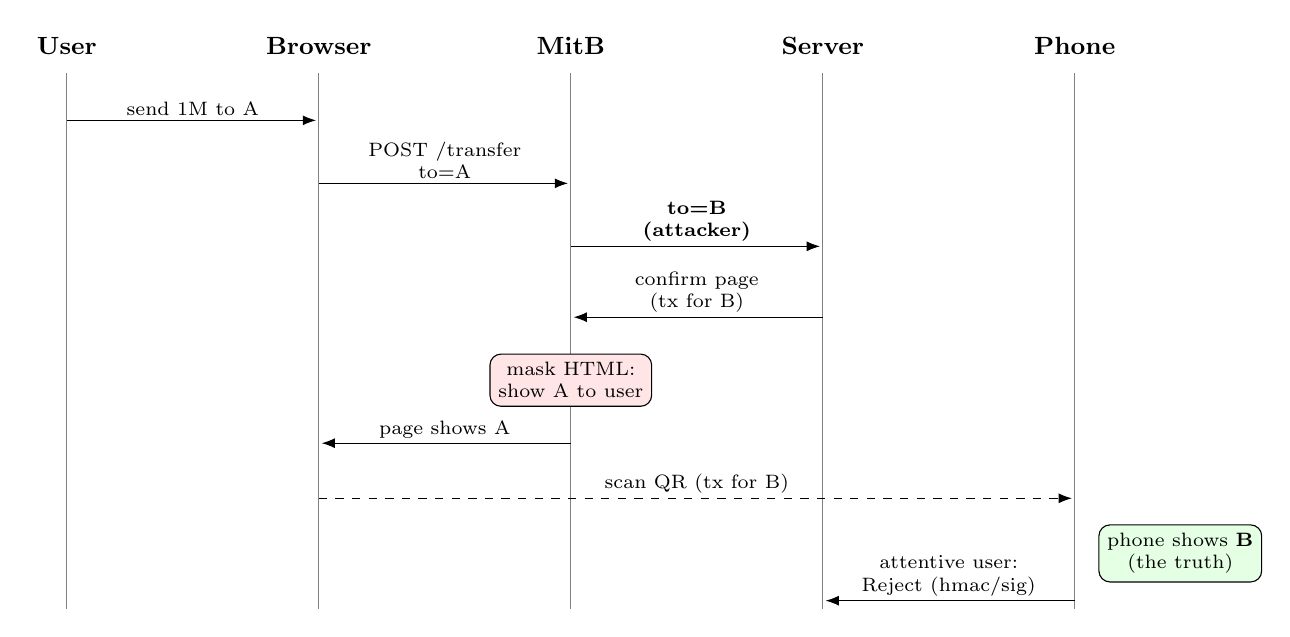
\begin{tikzpicture}[font=\small,>=Latex,
  msg/.style={->,shorten >=1pt},
  lab/.style={above,font=\scriptsize,fill=white,inner sep=1.5pt,align=center,midway},
  note/.style={align=center,font=\scriptsize,draw,rounded corners,inner sep=3pt}]
  \foreach \x/\name in {0/User, 3.2/Browser, 6.4/MitB, 9.6/Server, 12.8/Phone}{
    \node[font=\small\bfseries] at (\x,0.35) {\name};
    \draw[gray] (\x,0) -- (\x,-6.8);
  }
  \draw[msg] (0,-0.6) -- node[lab]{send 1M to A} (3.2,-0.6);
  \draw[msg] (3.2,-1.4) -- node[lab]{POST /transfer\\to=A} (6.4,-1.4);
  \draw[msg] (6.4,-2.2) -- node[lab]{\textbf{to=B}\\\textbf{(attacker)}} (9.6,-2.2);
  \draw[msg] (9.6,-3.1) -- node[lab]{confirm page\\(tx for B)} (6.4,-3.1);
  \node[note,fill=red!10] at (6.4,-3.9) {mask HTML:\\show A to user};
  \draw[msg] (6.4,-4.7) -- node[lab]{page shows A} (3.2,-4.7);
  \draw[msg,dashed] (3.2,-5.4) -- node[lab]{scan QR (tx for B)} (12.8,-5.4);
  \node[note,fill=green!10,anchor=west] at (13.1,-6.1) {phone shows \textbf{B}\\(the truth)};
  \draw[msg] (12.8,-6.7) -- node[lab]{attentive user:\\Reject (hmac/sig)} (9.6,-6.7);
\end{tikzpicture}}
\caption{Confirmation under MitB. The browser is deceived, but the phone
reads the transaction the server holds, so \texttt{hmac}/\texttt{sig} expose the
swap. In \texttt{sig\_blind} the phone shows nothing and the user approves.}
\label{fig:confirm}
\end{figure}

\section{Reproducing the results}\label{app:repro}
The repository is a single project. With Python~3.11+ and Node~20+:
\begin{lstlisting}[language=bash]
python3 -m venv .venv && source .venv/bin/activate
pip install -e ".[dev]"
make test        # Python unit/integration tests
make test-js     # authenticator crypto vs shared/vectors.json
make eval        # scenarios + brute-force + benchmarks -> results/
\end{lstlisting}
All measured values come from files under \texttt{results/}:
\texttt{scenarios.csv} (\cref{tab:scenarios}), \texttt{bruteforce.csv} (online
guessing), \texttt{bench.csv}, \texttt{phone\_bench.csv} and \texttt{sizes.csv}
(performance), \texttt{screens/*.png} (\cref{fig:mitb}) and
\texttt{bench\_env.json} (host environment). The phone benchmarks and the
live-demo screenshots are collected by hand; the rest is produced by
\texttt{make eval}.

\section{Live man-in-the-browser demo}\label{app:mitb}
The screenshots in \cref{fig:mitb} were produced by running the attacker addon in
a proxy between a compromised browser and the server:
\begin{lstlisting}[language=bash]
pip install -e ".[attack]"            # mitmproxy into the venv (has segno)
make run MODE=sig                     # terminal 1
.venv/bin/mitmdump -s attacker/mitb_addon.py \
    --listen-port 8080 --ssl-insecure # terminal 2
# victim browser: proxy 127.0.0.1:8080, trust the mitmproxy CA (http://mitm.it)
# phone: connects to the server directly (not through the proxy)
\end{lstlisting}
Setting \texttt{MITB\_FORGE\_QR=1} also forges the QR to show the intended
recipient (scenario S4); the phone is then deceived, but the signature no longer
matches the transaction the server holds, so the bank rejects it.

\section{Demo accounts}\label{app:accounts}
\begin{table}[H]
\centering\small
\begin{tabular}{@{}lllr@{}}
\toprule
Username & Account & Name & Balance (VND) \\
\midrule
alice   & 0011223344 & NGUYEN VAN A & 100{,}000{,}000 \\
bob     & 0123456789 & TRAN THI B   & 5{,}000{,}000 \\
mallory & 0999888777 & LE VAN M     & 0 \\
\bottomrule
\end{tabular}
\end{table}
Passwords are hashed with scrypt ($n=2^{14}, r=8, p=1$). The symmetric keys are
stored in plaintext \emph{on purpose}, to make scenario S10 real; a production
system must use an HSM.


\end{document}
